% IMPORTANT
 
% Install tex distribution
% https://www.latex-project.org/get/
% With Windows, install MikTeX
 
% in RStudio, install.packages("knitR")
% also, install all packages that appear in first code chunk in this file, i.e. in the one that looks like this
% <<LoadingPackages, include=FALSE>>=
% library(knitr)
% library(xtable)
% library(dplyr)
% library(stargazer)
% library(cowplot)
% @

% Go to Tools/Global Options/Sweave
% Select Weave Rnw files using: knitr
% Select Typeset LaTeX into PDF using: pdfLaTeX
 
% Use button "Compile PDF" to knit the Rnw file to a tex file and compile the tex file to a pdf file.

% Always install all packages that you're asked to after having pressed "Compile PDF".
 
% If there is no error while knitting from Rnw to tex, but an error while compiling from tex to pdf, have a look at the pdf file. It might still have worked.

% instead of Compile PDF, go into Terminal and enter 
% Rscript -e "library(knitr); knit('paper.Rnw')"
% latexmk -pdf paper



% turn page 90 degrees with lscape Gandrud (2016), p.185

% Create clickable hyperlinks with hyperref package, Gandrud (2016), p. 218

% Use natbib package for bibliography formatting, authoryear for Harvard style , Gandrud (2016), p. 227
% commands to change what information is included in the parentheses, Gandrud (2016), p. 228, table 11.2

% Using saveRDS and readRDS, following 
% https://csgillespie.github.io/efficientR/efficient-inputoutput.html#efficient-data-export-.rdata-or-.rds

% working with knitR and LaTeX
% https://kbroman.org/knitr_knutshell/pages/latex.html

% rotate tables in knitr
% https://stackoverflow.com/questions/21840878/rotate-a-table-from-r-markdown-in-pdf
% in particular stargazer tables
% https://stackoverflow.com/questions/31169845/rotate-stargazer-table-in-knitr/34292292#34292292

% Create list of packages used, Gandrud (2016), p 218/219



% models with robust standard errors texreg
% https://github.com/DeclareDesign/estimatr/issues/316

\documentclass[12pt, a4paper, titlepage]{article}\usepackage[]{graphicx}\usepackage[]{color}
% maxwidth is the original width if it is less than linewidth
% otherwise use linewidth (to make sure the graphics do not exceed the margin)
\makeatletter
\def\maxwidth{ %
  \ifdim\Gin@nat@width>\linewidth
    \linewidth
  \else
    \Gin@nat@width
  \fi
}
\makeatother

\definecolor{fgcolor}{rgb}{0.345, 0.345, 0.345}
\newcommand{\hlnum}[1]{\textcolor[rgb]{0.686,0.059,0.569}{#1}}%
\newcommand{\hlstr}[1]{\textcolor[rgb]{0.192,0.494,0.8}{#1}}%
\newcommand{\hlcom}[1]{\textcolor[rgb]{0.678,0.584,0.686}{\textit{#1}}}%
\newcommand{\hlopt}[1]{\textcolor[rgb]{0,0,0}{#1}}%
\newcommand{\hlstd}[1]{\textcolor[rgb]{0.345,0.345,0.345}{#1}}%
\newcommand{\hlkwa}[1]{\textcolor[rgb]{0.161,0.373,0.58}{\textbf{#1}}}%
\newcommand{\hlkwb}[1]{\textcolor[rgb]{0.69,0.353,0.396}{#1}}%
\newcommand{\hlkwc}[1]{\textcolor[rgb]{0.333,0.667,0.333}{#1}}%
\newcommand{\hlkwd}[1]{\textcolor[rgb]{0.737,0.353,0.396}{\textbf{#1}}}%
\let\hlipl\hlkwb

\usepackage{framed}
\makeatletter
\newenvironment{kframe}{%
 \def\at@end@of@kframe{}%
 \ifinner\ifhmode%
  \def\at@end@of@kframe{\end{minipage}}%
  \begin{minipage}{\columnwidth}%
 \fi\fi%
 \def\FrameCommand##1{\hskip\@totalleftmargin \hskip-\fboxsep
 \colorbox{shadecolor}{##1}\hskip-\fboxsep
     % There is no \\@totalrightmargin, so:
     \hskip-\linewidth \hskip-\@totalleftmargin \hskip\columnwidth}%
 \MakeFramed {\advance\hsize-\width
   \@totalleftmargin\z@ \linewidth\hsize
   \@setminipage}}%
 {\par\unskip\endMakeFramed%
 \at@end@of@kframe}
\makeatother

\definecolor{shadecolor}{rgb}{.97, .97, .97}
\definecolor{messagecolor}{rgb}{0, 0, 0}
\definecolor{warningcolor}{rgb}{1, 0, 1}
\definecolor{errorcolor}{rgb}{1, 0, 0}
\newenvironment{knitrout}{}{} % an empty environment to be redefined in TeX

\usepackage{alltt}
\usepackage{lscape}
\usepackage{graphicx}
\usepackage[utf8]{inputenc}
\usepackage[backend=biber, bibstyle=apa, citestyle=authoryear]{biblatex}
\usepackage{floatrow}
\usepackage{booktabs}
% \usepackage{bookmark}
\usepackage{rotating}
\usepackage{dcolumn}
% \usepackage[authoryear]{natbib}
% \bibliographystyle{apalike}
\usepackage{mathtools}
% \usepackage[onehalfspacing]{setspace}
\usepackage[left = 2.5cm, top = 2.5cm, right = 2.5cm, bottom = 2.0cm]{geometry}
\usepackage[hidelinks]{hyperref}

% 1.5 spacing in Word is about this in LaTeX
% https://tex.stackexchange.com/questions/65849/confusion-onehalfspacing-vs-spacing-vs-word-vs-the-world

\linespread{1.25}

\addbibresource{references.bib}






% multiple authors
% https://tex.stackexchange.com/questions/4805/whats-the-correct-use-of-author-when-multiple-authors

\title{Analysis of survey data collected by CHILDREN for a better World e.V.}
\author{
Laura Huber\\
\texttt{11709507}
\and
Laura Jepsen\\
\texttt{11567799}
\and
Jonathan Kirschner\\
\texttt{11724530}
\and
Rafael Schütz\\
\texttt{11574909} 
\and 
Yannick Zurl\\
\texttt{11701793}
\and
Studentisches Praxisprojekt zur Empirischen Wirtschaftsforschung PaRE3To\\
\and
Ludwig-Maximilians-Universität Munich
}

% Winter Term 2019/20\\

\date{27th February 2020}
\IfFileExists{upquote.sty}{\usepackage{upquote}}{}
\begin{document}

% \begin{titlepage}
\maketitle
% \end{titlepage}

\tableofcontents
\listoftables

% note below table
% https://stackoverflow.com/questions/44549464/table-spacing-issue-converting-to-pdf-via-latex-with-pandoc/44797387#44797387
\listoffigures

\begin{abstract} 
This study describes the analysis of the data from the non-profit organisation 'CHILDREN for a better world e.V.'. We obtain null-results associated to the subsidy CHILDREN provides for its two flagship programs, Meals and Trips, and selected outcome variables. We find a strong but only partially robust connection between health relevant outcomes and the index of healthy diet criteria fulfilled in organization's menus. Using a differences-in-differences strategy, we cannot show a significant effect of participating in the trips program on the everyday expertise and selfworth of the beneficiaries.
\end{abstract}

\section{Introduction}

CHILDREN supports organizations working with children and youth across Germany (in German: Einrichtungen der offenen Kinder- und Jugendarbeit) across Germany. We call them organizations in the following. They apply to CHILDREN for yearly grants. If approved, they are supposed to use them for specific purposes defined by CHILDREN. CHILDREN provided us with data from two of its flagship programs: Mittagstisch (we refer to this as Meals program) and Entdeckerfonds (Trips program). The organizations use money from the Meals program to finance meals, from breakfast to dinner, that they sell at concessionary prices to the children and youth that visit them. In the following, we call these children and youth who ultimately profit from CHILDREN's grants beneficiaries. The organizations also use money from the Trips program to make trips to nearby places usually unknown to the beneficiaries.  
Unless otherwise specified, we consider all variables to be metric, even if they are ordinal. 

Previous research shows, that the childhood and youth is central in development of character traits and future opportunities. Factors like education, stable family conditions, social contacts and mobility shape children and adolescents for their further life. Children from parents with lower income and lower educational attainment have typically a lower weight at birth and are born in a later week of gestation, which are indicators for bad initial conditions, as shown by \textcite{Case.2002}. Children which grow up in families with a low socio-economic status are often less mobile and more likely to stay amongst themselves. This could have a negative influence on their character development. For example, \textcite{Chetty.2014} investigate for the US, that areas with more mobility are highly correlated with better primary schools, greater social capital and more stable family conditions. Furthermore, the result of \textcite{Kosse.2020} provides causal evidence on the effect of social environment on prosocial attitudes. Being supported by a mentor could result in a significant and persistent increase in the prosociality of elementary school children, with regard to prosocial role models and intense social interactions. \textcite{Heckman.2010} investigated a preschool education program in the US. He shows that an investment in the improvement of the childhood conditions could have a high rate of return, even by controlling for possible distortions.   

CHILDREN for a better World e.V. is a non-profit organization supporting social institutions for children and adolescents across Germany, such as youth centers. Their goal is to foster equality of opportunities for the youth in Germany. CHILDREN supports poor and disadvantaged families and young people in socially problematic areas. Furthermore, they fight child poverty and encourage the youth to engage in society. We call the institutions funded by CHILDREN organizations in the following. Organizations have to apply for funding from CHILDREN each year again. In the application process, CHILDREN requires the applicants to answer a survey which contains questions about outcomes related to CHILDREN’s programs as well as general information about the organization such as the yearly budget.
CHILDREN provided us with data from two of its flagship programs: Mittagstisch (we refer to this as Meals program) and Entdeckerfonds (Trips program). The organizations use money from the Meals program to finance meals, from breakfast to dinner, that they sell at concessionary prices to the children and adolescents that visit them. In the following, we call these children and youth who ultimately profit from CHILDREN's grants beneficiaries. The organizations also use money from the Trips program to make trips to nearby places usually unknown to the beneficiaries.  

Previous research shows that childhood and youth are central in the development of character traits and future opportunities. Factors like education, stable family conditions, social contacts and mobility shape children and adolescents for their further life. Heckmann and Carneiro (2003) show that especially early family factors determine most of the gaps in high school attendance. Moreover, Deckers et. al. (2015) found, by experiments conducted in Germany, that children of higher educated parents are significantly more patient. Children from parents with lower income and a lower educational level typically have a lower weight at birth and are born in a later week of gestation, which are all indicators for bad initial conditions (Deckers et. al. 2015, Case et. al. 2002). Children that grow up in families with a low socio-economic status are often believed to be less mobile. This could have a negative influence on their character development. For example, Chetty et. al (2012) investigate for the US, that areas with more mobility are highly correlated with better primary schools, greater social capital and more stable family conditions. Furthermore, the results of Deckers et. al. (2020) provide evidence for the effect of the social environment on prosocial attitudes. Being supported by a mentor could result in a significant and persistent increase in the prosociality of elementary school children. Heckmann et. al. (2010) investigated a preschool education program in the US. The authors show that an investment in the improvement of the childhood conditions could have a high rate of return, even after controlling for possible distortions. 

The aim of our project paper is to test whether CHILDREN’s programs positively influence the beneficiaries. We look at the associations between the subsidy CHILDREN provides and the share of beneficiaries with broadened everyday expertise and improved selfworth. Furthermore, we analyze the association between the measure of the healthiness of the meals the organizations offer and health-relevant outcomes of beneficiaries. The aim of our applied differences-in-differences estimation is to test whether the activities offered by the trips program have a positive effect on the participating children, measured through a change in selfworth and everyday expertise.
We find no profound connection between the subsidy CHILDREN provides and the effectiveness of the organizations regarding the share of beneficiaries with broadened everyday expertise and improved selfworth. On the other hand, focusing on health relevant variables, we obtain a positive association between the index of healthy diet criteria fulfilled by organizations and the share of beneficiaries who are less frequently ill. By using the differences-in-differences (DID) strategy, the estimates show that the participation in the trips program has a positive, but insignificant effect on the everyday expertise of beneficiaries. Strikingly, we observe a negative association between participating in the trips program and selfworth. However, the results of the DID estimation should not be overstated because of the small sample size.
The remainder of this project paper is structured as follows: Section \ref{data} describes the variable used for the empirical analysis. Then we present summary statistics. We explain the dimensionality reducing method factor analysis. The proceeding section reports different regression results. After that, we implement the differences-in-differences strategy to test for the effects of the trips program. Finally, we conclude and provide suggestions for CHILDREN.

\section{Data}
\label{data}

To measure the effect of CHILDREN's programs on the supported organizations, we use data from 2011 to 2018. In each year CHILDREN sends a survey to the organizations with several questions about the previous year. The number of organizations varies across years and increases over time: From 52 organizations in 2011 to 68 organizations in 2018. In some organizations one specific employee answers the survey questions, while in other institutions the questionnaire is answered in a team. As the children and adolescents are not questioned directly, all responses are documented as perceptions of the employees. The constellation of the variables in the data set also varies across years. For instance, CHILDREN asks for the average amount of kids that increased their confidence or improved their dietary knowledge. These questions of the survey are based on a scale of five levels from no to all kids. We perform several steps to receive a full dataset, which we use in our empirical analysis. Originally, the data was divided into seperate data sets for the respective years. We only use the surveys until 2018, because in 2019 some organization-ID's occurred multiple times and the dataset for 2019 was incomplete. To ensure comparability across years, we named all variables the same. We merged the different datasets to a common dataset, including all years and variables CHILDREN collected. For an efficient and clear data structure, we created a function that automatically changed the data type of all variables from "character" to "ordinal" and added several versions for each initially metric encoded variable afterwards. The three variants are ordinal, standardized and weighted.
Furthermore, we created a set of new variables. For instance, we used the information CHILDREN gave us to assign the German states to the corresponding organization-ID. 
The final dataset for the empirical analysis is structured as follows: Each row represents a specific organization observed in a specific year. The questions are divided in two categories. The first part of the data set includes variables regarding the meals program. The second part contains variables affecting the trips program. The final data set comprises the years 2011 to 2018.
Many organizations do not answer all questions CHILDREN poses. We create a seperate data set, in which we impute missing values with an organization-specific linear trend. CHILDREN supports some very large organizations that give out hundreds of meals a day or conduct dozens of trips per year. We fit our models with outliers excluded to see if they are driving results. We define an outlier as a value that is at least 1.5 interquartile ranges below the 25th percentile or equally far above the 75th percentile. Once we exclude outliers in terms of numbers of meals and once in terms of number of trips.

\section{Summary Statistics}
\subsection{Fundamental Dynamics} 

In this section, we give an overview of the dynamics of CHILDREN's two flagship programs. We focus on the number of estimated ultimate beneficiaries in both programs, median total subsidy, median subsidy per institution, and median subsidy per beneficiary. We also look at selected outcomes, i.e. those related to health as well as self-worth and day-to-day skills. We have converted all nominal monetary variables into 2015 euros, using price indices from the Federal Statistical Office of Germany (Statistisches Bundesamt). We deflate (requested) grants as well as organizations' total expenses for the Meals program  with the price index related to food and non-alcoholic beverages (in German: Nahrungsmittel und alkoholfreie Getränke) and (requested) grants towards the Trips program with the price index for leisure, entertainment, and culture (in German: Freizeit, Unterhaltung und Kultur). These are only available after logging in on DESTATIS. The organizations also gave information about their total yearly budget. We inflate this with the general price index.


<<<<<<< HEAD
% latex table generated in R 3.6.2 by xtable 1.8-4 package
% Sat Feb 29 17:56:41 2020
=======
% latex table generated in R 3.5.1 by xtable 1.8-4 package
% Sat Feb 29 17:58:47 2020
>>>>>>> b24662a116b8b0301ff26431155b33d6392d6dc5
\begin{table}[ht]
\centering
\begin{tabular}{lccccc}
  \hline
 & Year & Beneficiaries, Meals & Beneficiaries, Trips & Organizations, Meals & Organizations, Trips \\ 
  \hline
1 & 2011 & 3748.0 &  & 52 &  \\ 
  2 & 2012 & 3556.0 & 2803.0 & 51 & 44 \\ 
  3 & 2013 & 4015.0 & 2823.0 & 55 & 42 \\ 
  4 & 2014 & 4685.0 & 2752.0 & 55 & 43 \\ 
  5 & 2015 & 5857.0 & 3823.0 & 55 & 49 \\ 
  6 & 2016 & 3075.0 & 3819.0 & 59 & 48 \\ 
  7 & 2017 & 4895.0 & 4150.0 & 64 & 48 \\ 
  8 & 2018 & 5102.5 & 6911.0 & 68 & 49 \\ 
   \hline
\end{tabular}
\caption{Summary Statistics} 
\label{fundamentalDynamics}
\end{table}

% look up official names of price indices in English 


Table \ref{fundamentalDynamics} shows that, at the beginning of the time series in 2011, in the Lunch program they supported in 52 organizations. In 2018, this number has increased to 68. In 2011, CHILDREN financed meals for 3748 beneficiaries, and for 5103 in 2018. In the trips program, which launched in 2012, the number of supported organizations amounted to 44 in 2012 and grew to 49 until 2018. In 2012, their grant allowed 2803 beneficiaries to go on trips, and 6911 in 2018.

\subsection{Trends of grants} 

\begin{figure}
  \caption{Yearly dynamics of total grants in Meals and Trips program}
  \label{totalGrantsDyn}

\begin{knitrout}
\definecolor{shadecolor}{rgb}{0.969, 0.969, 0.969}\color{fgcolor}

{\centering 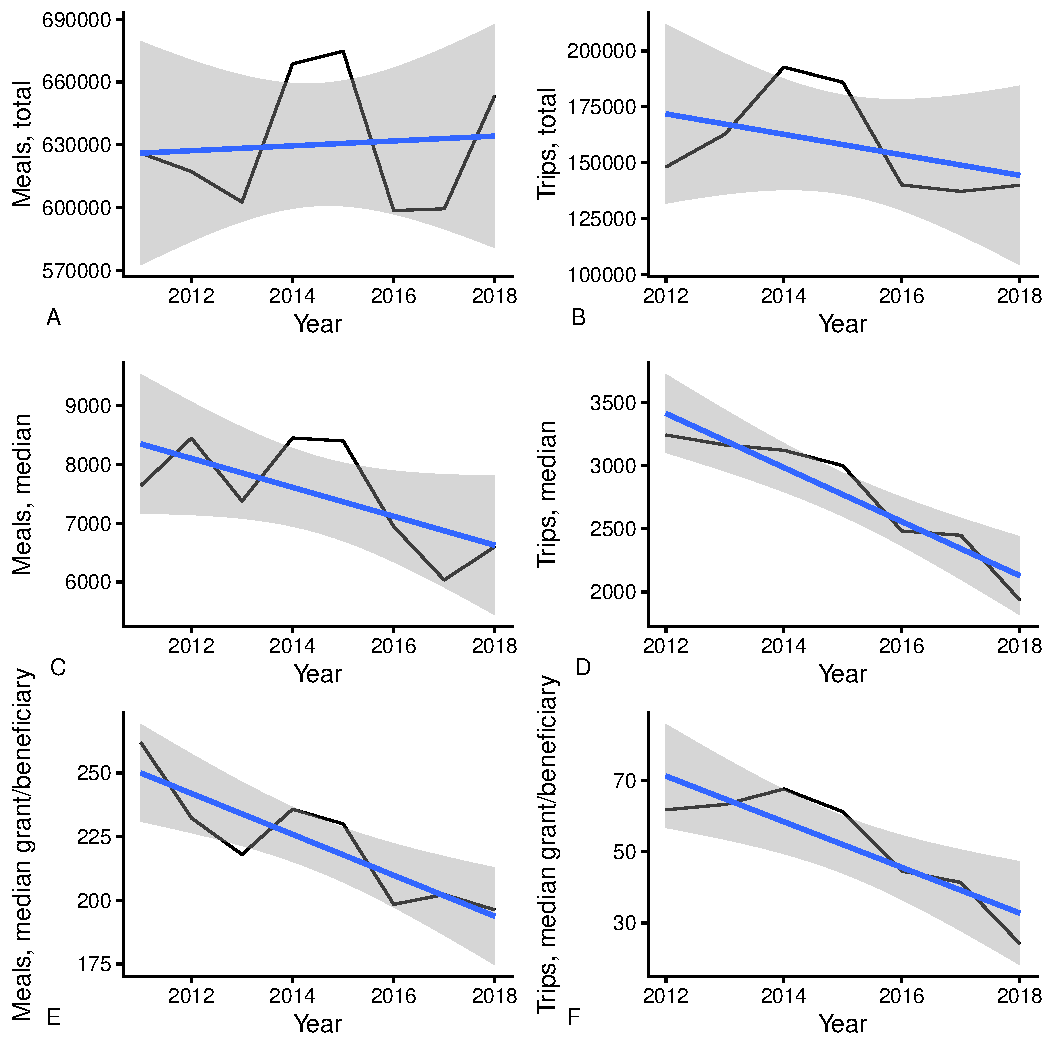
\includegraphics[width=0.8\textwidth]{figure/GrantTrend-1} 

}



\end{knitrout}

\floatfoot{This graph shows the development of grants in the Meals compared to the Trips program. We distinguish between the sum of grants in one year, the median grant and the median grant per beneficiary. From left to right: Meals, Trips. From top to bottom: sum, median, median per beneficiary. We have deflated the values to 2015 euros using the price index related to food and non-alcoholic beverages(in German: Nahrungsmittel und alkoholfreie Getränke) for the Meals program and the price index related to Leisure, Entertainment and Culture (in German: Freizeit, Unterhaltung, Kultur) provided by the Federal Statistical Office of Germany (Statistisches Bundesamt).}
\end{figure}

For the dynamics of figure \ref{totalGrantsDyn} we visualze the dynamics of CHILDRENs' grants by distinguishing between the sum of grants in one year, the median and the median grant per beneficiary. We also compare the grants of the Lunch and the Trips Program.

Figure \ref{totalGrantsDyn} shows no exact trend for the total real grant for the Lunch program. Between 2013 and 2015 the grant increased from about 600000 EUR to 680000 EUR, but falls behind in the following year. Since 2017 an increase is again visible. In comparison to this, there is a clearer negative trend in median Meals subsidy, falling from about 8000 EUR in 2012 to about 6500 EUR in 2018. In accordance, the median Meals grant per beneficiary shrinks from about 250 EUR to about 200 EUR. 

In the total Trips grant, a slightly negative trend is visible, after the subsidy increased to approximately 200000 EUR in 2014, but decreased to about 130000 EUR in 2016, and is connstand eversince. The Trips median grant therefore also decreased from 3000 EUR to 2000 EUR over the time period, as well as the median grant per beneficiary decreased from about 60 EUR to about 30 EUR.

These results visualize, for the Lunch as well as for the Trips program, together with the fundamental dynamics of table \ref{fundamentalDynamics}, that children was able to increase the number of organizations they support, but had to distribute the available subsidy among them. 

\subsection{Dynamics of Health-Related Variables} 

In its yearly surveys, CHILDREN asks about three variables closley related to a healthy diet. These are the shares of beneficiaries who are healthier, have a growing appreciation for a healthy diet, or have increased their knowledge about what constitutes a healthy diet. Figure \ref{HealthTimeplots} displays the share of organizarions in each category of the health outcome from 2011 to 2018. The possible values are: all, most, some, few, and none. For this figure, we use the original ordinal varibles which result from the survey structure.  

\begin{figure}
  \caption{Health outcome over time}
  \label{HealthTimeplots}
\begin{knitrout}
\definecolor{shadecolor}{rgb}{0.969, 0.969, 0.969}\color{fgcolor}

{\centering 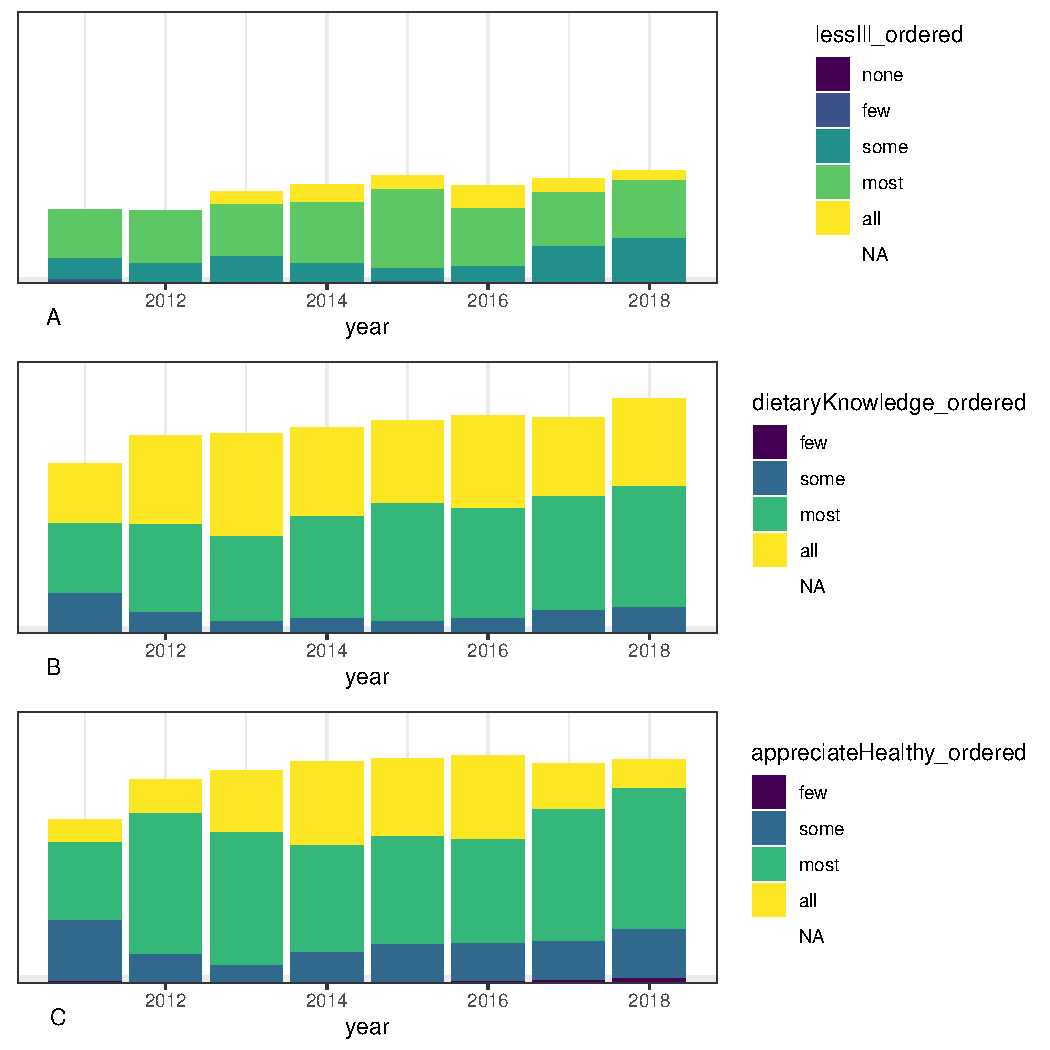
\includegraphics[width=0.8\textwidth]{figure/HealthTimePlots-1} 

}



\end{knitrout}
\floatfoot{In its yearly surveys CHILDREN asks about three variables closley related to a healthy diet. These are the shares of beneficiaries who are less frequently ill (lessIll\_ordered), with expanded dietary knowledge (dietaryKnowledge\_ordered), or with increased appreciation for a healthy diet (appreciateHealthy\_ordered).
The x-axis plots the year. The y-axis displays the share of organizarions in each category of the health outcome. The possible values are: all, most, some, few and none.}
\end{figure}

In Figure \ref{HealthTimeplots}, for the variable 'lessIll\_ordered', there is much non available data (lessIll\_ordered refers to the share of beneficiaries who are less frequently ill). In all years, most organizations say that most beneficiaries are more healthy. The least stated category is, that all beneficiaries are less ill. That few are less ill, appears sometimes and the leftover category, none, which is only coded for the variable 'lessIll\_ordered', appears as good as never.

In the second plot of figure \ref{HealthTimeplots} (variable 'dietaryKnowledge\_ordered', refers to the share of beneficiaries with expanded dietary knowledge) most organizations state, that predominantely most or all beneficiaries increased their knowledge about what constitutes a healthy diet. The least stated category is that some beneficiaries increased their dietary knowledge. The leftover category, few, does not appear.

The the bottom plot of figure \ref{HealthTimeplots}, which visualizes the variable 'appreciateHealthy\_ordered' (refers to the share of beneficiaries with increased appreciation for a healthy diet). Again most organizations state, that most beneficiaries have a growing appreciation for a healthier diet. The second most stated answer is that all beneficiaries have a growing appreciation for a healthier diet. The least stated category by the organizations is, as well as in the second plot, that some have a growing appreciation for a healthier diet. The leftover category, few, also does not appear.


\subsection{Selfworth and everyday expertise} 

In its yearly surveys, CHILDREN has always asked about the following two variables. These are the shares of beneficiaries with improved self-worth and with broadened everyday expertise. Figure 4 displays the share of organizarions in each category of the health outcome from 2011 to 2018. The possible values are: all, most, some, few, and none. As well as in the last figure (figure 3), we use the original ordinal varibles which result from the survey structure.

\begin{figure}
  \caption{Selfworth and everyday expertise over time}
  \label{EqualityTimeplots}
\begin{knitrout}
\definecolor{shadecolor}{rgb}{0.969, 0.969, 0.969}\color{fgcolor}

{\centering 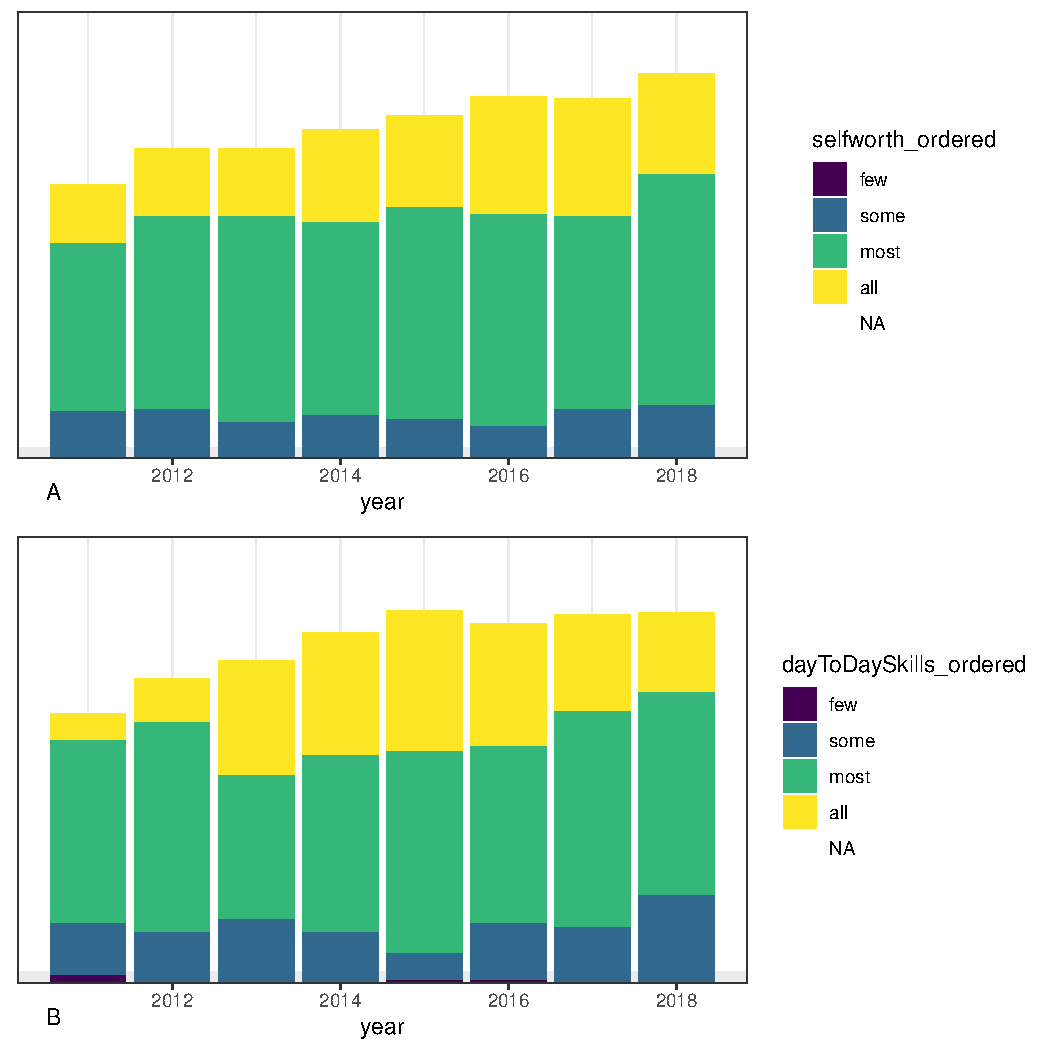
\includegraphics[width=0.8\textwidth]{figure/EqualityTimePlots-1} 

}



\end{knitrout}
\floatfoot{In its yearly surveys CHILDREN has always asked about following two variables. These are the shares of beneficiaries with improved self-worth (selfworth\_ordered) and with a broadened understanding for everyday expertise (dayToDaySkills\_ordered).
The x-axis plots the year. The y-axis displays the share of organizations in each category of the health outcome. The possible values are: all, most, some, few, and none.}
\end{figure}

Figure \ref{EqualityTimeplots} shows in its upper plot the development of the answered categories for the variable selfworth\_ordered (refers to the share of beneficiaries with improved self-worth). Mostly, the answer is that most beneficiaries in most organizations have more selfworth. The second most stated category is that all beneficiaries gained in selfworth and the least stated is that some have more selfworth. The leftover category, few, does not appear.

In the bottom plot of figure \ref{EqualityTimeplots} the development of the share of beneficiaries with a broadened understanding for everyday expertise over time is visible. The results are about similar to the previous results of selfworth: Most beneficiaries in most organisations have a growing understanding for everyday expertise. 

\section{Feature Selection}

CHILDREN survey many variables, some of which seem closely related to each other. We use exploratory factor analysis for dimensionality reduction and employ extracted factors as controls in the models we estimate. In the appendix, we use the partition method suggested by \textcite{Millstein.2020} to establish a one-to-one correspondence between apparent and underlying variables.

\subsection{Exploratory Factor Analysis}

The fundamental theorem of factor analysis posits that each observable variable can be expressed as a linear combination of a smaller number of underlying factors as well as an error term. The coefficients of the factors are called loadings. \parencite[p.310]{Moosbrugger.2008} 

For factor analysis, we work with the imputed data set. We conduct a separate factor analysis for each model that we want to fit. Each time, we include all variables that were recorded in all years the Meals and the Trips program have been run respectively, but exclude those that we want to use as response and predictor in the corresponding model. 

First, we determine the optimum number of factors via the stochastic approach of parallel analysis, following the advice of \textcite[p.313]{Moosbrugger.2008}.
We estimate factor scores and loadings with the Bartlett method, which is similar to a Maximum Likekelihood estimation, and presented as the most convential one in \textcite[p.291]{Eid.2014}.
As the fundamental theorem of factor analysis has no unique solution, we have to decide on how to rotate the factors. As we want them to be orthogonal to each other, we use the rotation technique Varimax, which is recommended for this purpose in \textcite[p.317]{Price.2017}. 

% \subsection{Double Selection}

\section{Associations Between CHILDREN's Grants and Selected Outcomes}

\subsection{Empirical Approach} 

In this section, we use a simple linear model, as described in equation \ref{SimpleLinearModel}. We estimate each model with the original data set, the one with imputed variables, and the one with excluded outliers. When appropriate, we include the relevant extracted factors as controls. 

\begin{equation}
\label{SimpleLinearModel}
  y_{it} = \beta_0 + \beta_1 x_{it} + \epsilon_{it}
\end{equation}

 We look at the association between: 

\begin{itemize}
  \item{the subsidy (in 2015 EUR) an organization receives through CHILDREN's Meals program and the number of meals it dispenses}
  \item{the subsidy (in 2015 EUR) an organization receives through CHILDREN's Trips program and the number of trips it conducts}
  \item{the subsidy per beneficiary (in 2015 EUR) an organization receives through CHILDREN's Meals program and the standardized share of beneficiaries with improved self-worth}
  \item{the subsidy per beneficiary (in 2015 EUR) an organization receives through CHILDREN's Meals program and the standardized share of beneficiaries with broadened everyday expertise}
   \item{a standardized measure of the healthiness of the meals an organization dispenses and various standardized health-related outcomes of beneficiaries} 
\end{itemize}

We discuss all these models in turn.

\subsection{Direct Effects of CHILDREN's Grants} 

If CHILDREN's grants are to have an effect on beneficiaries, they should first influence the output of organizations in terms of meals dispensed and trips conducted. 


\begin{table}
\caption{Association between number of meals and real subsidy}
\begin{center}
\scalebox{0.8}{
\begin{tabular}{l c c c c c}
\toprule
 & (1) & (2) & (3) & (4) & (5) \\
\midrule
(Intercept)     & $-12089.14^{*}$ & $-1814.16$     & $3535.39^{***}$ & $3107.70^{***}$ & $-12250.60^{**}$ \\
                & $(5192.86)$     & $(1765.93)$    & $(498.99)$      & $(508.94)$      & $(4524.09)$      \\
realSubsidy     & $2.61^{***}$    & $0.50^{**}$    & $0.29^{***}$    & $0.25^{***}$    & $2.72^{***}$     \\
                & $(0.57)$        & $(0.18)$       & $(0.05)$        & $(0.05)$        & $(0.51)$         \\
eatersPerMealNo &                 & $172.83^{***}$ &                 & $19.00^{*}$     &                  \\
                &                 & $(14.92)$      &                 & $(8.45)$        &                  \\
\midrule
R$^2$           & $0.43$          & $0.73$         & $0.13$          & $0.21$          & $0.45$           \\
Adj. R$^2$      & $0.43$          & $0.73$         & $0.12$          & $0.20$          & $0.45$           \\
Num. obs.       & $329$           & $329$          & $250$           & $250$           & $440$            \\
RMSE            & $39992.79$      & $27390.90$     & $3629.72$       & $3463.66$       & $39601.41$       \\
\bottomrule
\multicolumn{6}{l}{\scriptsize{\parbox{\linewidth}
{\vspace{2pt} Dependent variable: number of meals \\ realSubsidy: subsidy for Meals program in 2015 EUR \\ eatersPerMeal: number of beneficiaries of Lunch program \\ Model (1): original data set, simple linear model, estimated with OLS \\ Model (2): original data set, linear model with controls, estimated with OLS \\ Model (3): data set without outliers, simple linear model, esmitaed with OLS \\ Model (4): data set without outliers, linear model with controls, estimated with OLS \\ Model (5): imputed data set, simple linear model, estimated with OLS \\ All regressions are estimated with robust standard errors $^{***}p<0.001$; $^{**}p<0.01$; $^{*}p<0.05$.}}}
\end{tabular}
}
\label{GrantsRegressionsLunch}
\end{center}
\end{table}


As table \ref{GrantsRegressionsLunch} shows, this is emphatically true. Whether we look at the original data set, the one without outliers and the one with imputed values, a strong association becomes evident. 
The estimated coefficients are very similar when we use the original dataset and the one with imputed values. In the case of the original data set, increasing the subsidy to an organization by one EUR is associated with 2.6 additional meals dispensed. This estimate is highly statistically significant. When we exclude outliers, i.e. those organizations that give out very many menus or very few menus,
the estimated coefficient decreases by about one order of magnitude. Still, spending not much more than three EUR more goes hand in hand with one extra meal. The estimate is also highly statistically significant.

In the remit of the Trips program, the picture looks much different. In the case of the original data set and the data set with imputed variables, an increase in the trips subsidy by 5000 EUR is needed for an extra trip. The coefficent of 0.0002 is statistically significant at the 5\% level. As soon as outliers are excluded, the coefficent changes to 0.0003, which is highly statistically significant. This means that, according to this model, at least 3000 EUR are needed for an additional trip.
In sum, there seems to be no clear connection between how much money CHILDREN gives to an organization and the number of trips it organizes. 


\begin{table}
\caption{Association between number of trips and real subsidy}
\begin{center}
\scalebox{0.8}{
\begin{tabular}{l c c c c c}
\toprule
 & (1) & (2) & (3) & (4) & (5) \\
\midrule
(Intercept)      & $3.7049^{***}$ & $3.4394^{***}$ & $2.6236^{***}$ & $2.3660^{***}$ & $3.6237^{***}$ \\
                 & $(0.3313)$     & $(0.3359)$     & $(0.2300)$     & $(0.2609)$     & $(0.3253)$     \\
realTripsSubsidy & $0.0002^{*}$   & $0.0001$       & $0.0003^{***}$ & $0.0003^{***}$ & $0.0002^{*}$   \\
                 & $(0.0001)$     & $(0.0001)$     & $(0.0001)$     & $(0.0001)$     & $(0.0001)$     \\
tripsKidsNo      &                & $0.0059$       &                & $0.0043$       &                \\
                 &                & $(0.0032)$     &                & $(0.0027)$     &                \\
\midrule
R$^2$            & $0.0474$       & $0.0729$       & $0.0880$       & $0.1241$       & $0.0504$       \\
Adj. R$^2$       & $0.0444$       & $0.0671$       & $0.0844$       & $0.1172$       & $0.0476$       \\
Num. obs.        & $322$          & $319$          & $257$          & $256$          & $334$          \\
RMSE             & $2.9565$       & $2.8967$       & $1.6981$       & $1.6579$       & $2.9310$       \\
\bottomrule
\multicolumn{6}{l}{\scriptsize{\parbox{\linewidth}
{\vspace{2pt} Dependent variable: number of trips \\ realTripsSubsidy: subsidy for Trips program in 2015 EUR \\ tripsKidsNo: number of beneficiaries of Trips program \\ Model (1): original data set, simple linear model, estimated with OLS \\ Model (2): original data set, linear model with controls, estimated with OLS \\ Model (3): data set without outliers, simple linear model, esmitaed with OLS \\ Model (4): data set without outliers, linear model with controls, estimated with OLS \\ Model (5): imputed data set, simple linear model, estimated with OLS \\ All regressions are estimated with robust standard errors $^{***}p<0.001$; $^{**}p<0.01$; $^{*}p<0.05$.}}}
\end{tabular}
}
\label{GrantsRegressionsTrips}
\end{center}
\end{table}


\subsection{Variables of interest: selfworth and everyday expertise} 

In their surveys, CHILDREN asks about two variables in both programs. These are the share of beneficiaries with improved self-worth and share of beneficiaries with broadened everyday expertise. This feature could potentially allow us to compare the two programs regarding their realtive effectiveness. Like always, we standardize the two outcome variables. As before, we can only make associational claims. We invariably find no clear-cut relationship between the subsidy per beneficiary and the two outcomes. In fact, no coefficent is statistically significantly differnent from zero at any of the usual levels. 
The four variables are recorded for each year in which the program was operative.
Tables \ref{SelfworthRegressions} and \ref{DayToDaySkillsRegressions} present the null results. 


\usepackage{graphicx}

\begin{table}
\caption{Association between selfworth and subsidy per beneficiary}
\begin{center}
\scalebox{0.8}{
\begin{tabular}{l c c c c c}
\hline
 & (1) & (2) & (3) & (4) & (5) \\
\hline
(Intercept)                    & $0.08$   & $0.12$   & $0.09$   & $0.12$   & $0.23^{*}$   \\
                               & $(0.09)$ & $(0.12)$ & $(0.09)$ & $(0.11)$ & $(0.11)$     \\
realSubsidyPerBeneficiary      & $-0.00$  &          & $-0.00$  &          & $-0.00$      \\
                               & $(0.00)$ &          & $(0.00)$ &          & $(0.00)$     \\
realTripsSubsidyPerBeneficiary &          & $-0.00$  &          & $-0.00$  &              \\
                               &          & $(0.00)$ &          & $(0.00)$ &              \\
ML1                            &          &          &          &          & $0.24^{***}$ \\
                               &          &          &          &          & $(0.06)$     \\
ML2                            &          &          &          &          & $0.37^{***}$ \\
                               &          &          &          &          & $(0.05)$     \\
ML3                            &          &          &          &          & $0.15^{***}$ \\
                               &          &          &          &          & $(0.04)$     \\
\hline
R$^2$                          & $0.00$   & $0.01$   & $0.00$   & $0.01$   & $0.30$       \\
Adj. R$^2$                     & $0.00$   & $0.01$   & $0.00$   & $0.01$   & $0.28$       \\
Num. obs.                      & $428$    & $184$    & $430$    & $187$    & $161$        \\
RMSE                           & $1.00$   & $1.00$   & $1.00$   & $1.00$   & $0.79$       \\
\hline
\multicolumn{6}{l}{\scriptsize{\parbox{\linewidth}
{\vspace{2pt} realSubsidyPerBeneficiary: subsidy per beneficiary of Meals program in 2015 EUR \\ realTripsSubsidyPerBeneficiary: subsidy per beneficiary of Trips program in 2015 EUR \\Model (1): dependent variable: share of beneficiaries with improved self-worth in the Lunch program, original data set, simple linear model, estimated with OLS \\ Model (2): dependent variable: share of beneficiaries with improved self-worth in the Trips program, original data set, simple linear model, estimated with OLS \\ Model (3): dependent variable: share of beneficiaries with improved self-worth in the Lunch program, imputed data set, simple linear model, estimated with OLS \\ Model (4): dependent variable: share of beneficiaries with improved self-worth in the Trips program, imputed data set, simple linear model, estimated with OLS \\ Model (5): dependent variable: share of beneficiaries with improved self-worth in the Lunch program, imputed data set, linear model with extracted factor scores as controls, estimated with OLS \\ All regressions are estimated with robust standard errors $^{***}p<0.001$; $^{**}p<0.01$; $^{*}p<0.05$.}}}
\end{tabular}
}
\label{SelfworthRegressions}
\end{center}
\end{table}



\usepackage{graphicx}

\begin{table}
\caption{Association between everyday expertise and subsidy per beneficiary}
\begin{center}
\scalebox{0.8}{
\begin{tabular}{l c c c c c c}
\hline
 & (1) & (2) & (3) & (4) & (5) & (6) \\
\hline
(Intercept)                    & $0.15$   & $0.13$   & $0.14$   & $0.11$   & $0.28^{*}$   & $0.08$       \\
                               & $(0.09)$ & $(0.10)$ & $(0.09)$ & $(0.10)$ & $(0.11)$     & $(0.09)$     \\
realSubsidyPerBeneficiary      & $-0.00$  &          & $-0.00$  &          & $-0.00$      &              \\
                               & $(0.00)$ &          & $(0.00)$ &          & $(0.00)$     &              \\
realTripsSubsidyPerBeneficiary &          & $-0.00$  &          & $-0.00$  &              & $-0.00$      \\
                               &          & $(0.00)$ &          & $(0.00)$ &              & $(0.00)$     \\
ML1                            &          &          &          &          & $0.31^{***}$ & $0.03$       \\
                               &          &          &          &          & $(0.06)$     & $(0.07)$     \\
ML2                            &          &          &          &          & $0.40^{***}$ & $0.16^{*}$   \\
                               &          &          &          &          & $(0.06)$     & $(0.07)$     \\
ML3                            &          &          &          &          & $0.16^{**}$  & $0.19^{**}$  \\
                               &          &          &          &          & $(0.05)$     & $(0.06)$     \\
ML4                            &          &          &          &          &              & $0.49^{***}$ \\
                               &          &          &          &          &              & $(0.06)$     \\
\hline
R$^2$                          & $0.01$   & $0.01$   & $0.01$   & $0.01$   & $0.37$       & $0.37$       \\
Adj. R$^2$                     & $0.01$   & $0.01$   & $0.01$   & $0.01$   & $0.36$       & $0.35$       \\
Num. obs.                      & $426$    & $177$    & $429$    & $181$    & $161$        & $169$        \\
RMSE                           & $1.00$   & $0.98$   & $1.00$   & $0.99$   & $0.78$       & $0.80$       \\
\hline
\multicolumn{7}{l}{\scriptsize{\parbox{\linewidth}
{\vspace{2pt} realSubsidyPerBeneficiary: subsidy per beneficiary of Meals program in 2015 EUR \\ realTripsSubsidyPerBeneficiary: subsidy per beneficiary of Trips program in 2015 EUR \\ Model (1): dependent variable: share of beneficiaries with with broadened everyday expertise in the Lunch program, original data set, simple linear model, estimated with OLS \\ Model (2): dependent variable: share of beneficiaries with with broadened everyday expertise in the Trips program, original data set, simple linear model, estimated with OLS \\ Model (3): dependent variable: share of beneficiaries with with broadened everyday expertise in the Lunch program, imputed data set, simple linear model, estimated with OLS \\ Model (4): dependent variable: share of beneficiaries with with broadened everyday expertise in the Trips program, imputed data set, simple linear model, estimated with OLS\\ Model (5): dependent variable: share of beneficiaries with with broadened everyday expertise in the Lunch program, imputed data set, linear model with extracted factor scores as controls, estimated with OLS \\ Model (6): dependent variable: share of beneficiaries with with broadened everyday expertise in the Trips program, imputed data set, linear model with extracted factor scores as controls, estimated with OLS \\ All regressions are estimated with robust standard errors $^{***}p<0.001$; $^{**}p<0.01$; $^{*}p<0.05$.}}}
\end{tabular}
}
\label{DayToDaySkillsRegressions}
\end{center}
\end{table}


\subsection{Variables of interest: Health variables} 

Now, we turn to a predictor that CHILDREN does not directly influence until now, but that it easily could. In 2014, 2016, 2017 and 2018 the organizations had to send CHILDREN a sample of their menus. An ecotrophologist collaborating with CHILDREN assessed those menus with regards to how healthy they were. This assessment was based on criteria of the German Nutrition Society (Deutsche Gesellschaft für Ernährung). 

In its yearly surveys, CHILDREN asks about three variables closely related to a healthy diet. These are the shares of beneficiaries who are less frequently ill, with expanded dietary knowledge and with increased appreciation for a healthy diet. 

Figure \ref{HealthPlots} gives an overview of the relationship between the healthy food criterion (DGECriteriaNo, index of healthy diet criteria fulfilled in organization's menu) and each of the three health-related variables. For these results, we use their ordinal values. The x-axis displays the index for a healthy diet. The y-axis displays the share of organizarions in each category of the health outcome. The possible values are: all, most, some, few and none. For example, if an organization says that most beneficiaries are healthier, then this would be coded as most. In the last reporting period, there are 13 healthy diet criteria. In previous years there were up to 15. The ecotrophologist assessed each criterion individually and decided wether it was fulfilled or not. The healthy food incex is calculated as the number of fulfilled criteria. Examples for criteria are daily carbohydrates or daily vegetables.  

All plots of Figure \ref{HealthPlots} show that most organizations suffice about 5 to 10 healthy food criteria. The largest part of criterion values are associated with most beneficiaries being less Ill, having a growing appreciation for a healthy diet or having increased their knowledge about what constitutes a healthy diet. It secondly becomes visible that the healthy criterion only exchanges with a growing appreciation for a healthy diet or an increasing dietary knowlege for all beneficiaries (which is the second most stated criterion in the two bottom plots), but not with all beneficaries being more healthy. However, for the variable less ill, the least data is availabe. Overall, the criteria, even a few, seem to have a positive relationship with beneficiaries health relevant variables. This connection is empiricaly examined in regressions \ref{HealthRegressions-LessIll}, \ref{HealthRegressions-DietaryKnowledge} and \ref{HealthRegressions-AppreciateHealthy}.

\begin{figure}
  \caption{Health Outcomes versus Healthy Meals}
  \label{HealthPlots}
\begin{knitrout}
\definecolor{shadecolor}{rgb}{0.969, 0.969, 0.969}\color{fgcolor}

{\centering 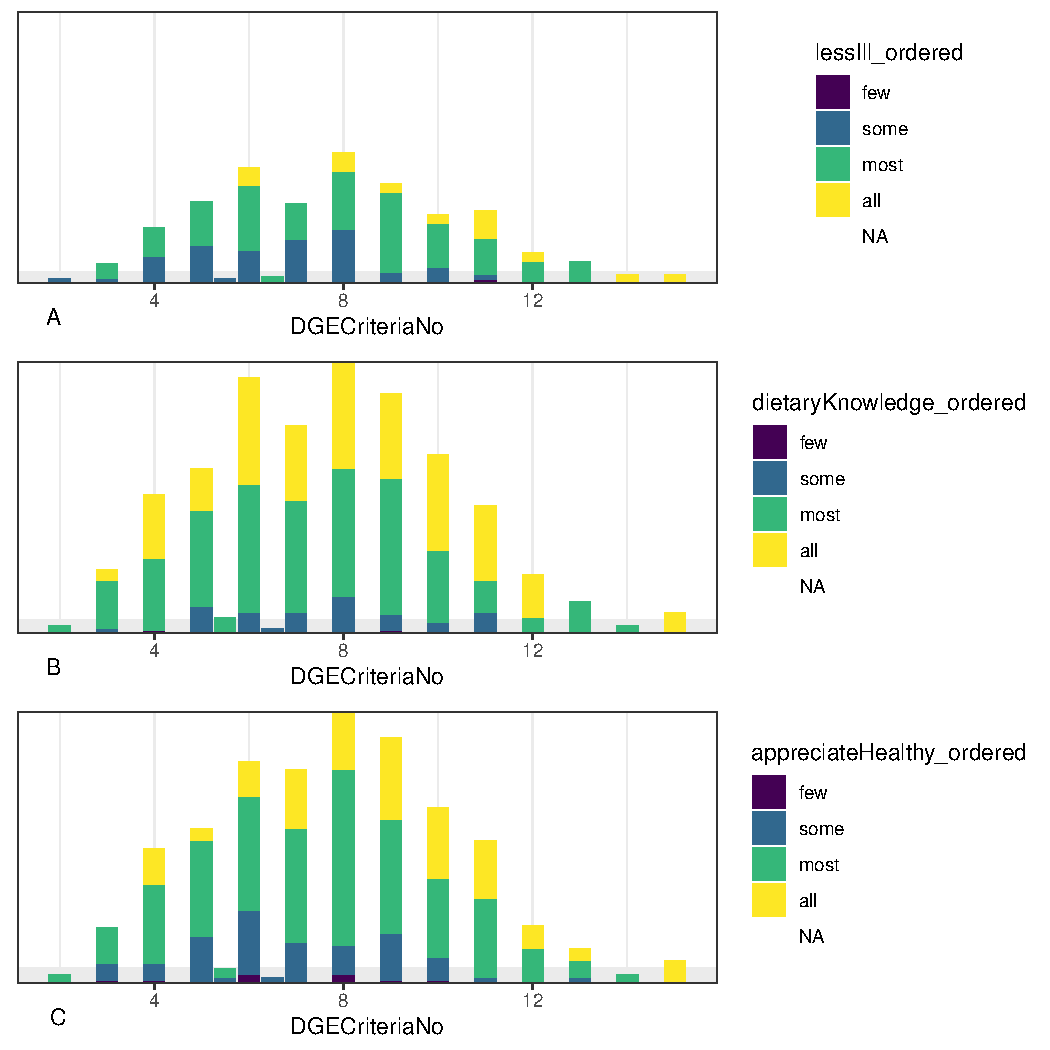
\includegraphics[width=0.8\textwidth]{figure/HealthRegressionsPercentageplots-1} 

}



\end{knitrout}
\floatfoot{DGECriteriaNo is an index of healthy diet criteria fulfilled in organization's menu. It is based on criteria of the German Nutrition Society (Deutsche Gesellschaft für Ernährung). According to information from CHILDREN, they ask the organizations to send them a sample of their menus. An ecotrophologist collaborating with CHILDREN assessed the menus. In its yearly surveys CHILDREN asks about three variables closley related to a healthy diet. These are the shares of beneficiaries who are less frequently ill (lessIll\_ordered), with expanded dietary knowledge (dietaryKnowledge\_ordered), or with increased appreciation for a healthy diet (appreciateHealthy\_ordered).
The x-axis plots the index for a healthy diet. The y-axis displays the share of organizarions in each category of the health outcome. The possible values are: all, most, some, few, and none}
\end{figure}

We use standardized versions of the health related variables as outcomes in simple linear models with a standardized version of the healthy food criterion as predictor in each.
By estimating these models with ordinary least squares (OLS), we ascribe the same weight to an organization where a thousand beneficiaries regularly eat as to one where only ten people do so. To control for this difference in size, we additionally fit the models with weighted least squares (WLS), using the number of beneficiaries as weights.

In Table \ref{HealthRegressions-LessIll}, after weighting the regression for the original data set, the coefficent rises slightly but is becoming less statistically significant. An increase of the healthy food criterion by one standard deviation is associated with an increase in beneficiaris being less frequently ill by 0.35 standard deviations. Regressing with the imputed dataset, results decrease by about 0.1. Using weighted least squares additionaly results in a slighty decreased coefficent, which is not significant anymore. Regressing with the imputed data set with extracted factor scores as controls, we still obtain a slightly postive significant coefficent: An increase of the healthy food criterion by one standard deviation is associated with an increase in beneficiaris being less frequently ill by 0.18 standard deviations. Overall, there is a positive association between the two variables.    

An expanded model with the dependent variable less Ill is presented in Appendix 1 in table \ref{expandLessIll}. 

In Table \ref{HealthRegressions-DietaryKnowledge} weighted least squares constanly leads to smaller coefficents which are not statistically significant. For the original data set, the coeffiecent is slightly negative. Using the imputed data set, an increase in the healthy meals criterion by one standard deviation is associated with an increase in beneficiaries dietary knowledge by 0.l standard deviations. This coefficent is as well insignifacant. Also, regressing with the imputed data set with extracted factor scores as controls, does not display a profound connection between beneficiaries dietary knowledge and the healthy meals index.  

In the regressions presented in table \ref{HealthRegressions-AppreciateHealthy}, the changes between ordinary and weíghted least squares are much stronger. For the original data set, the OLS coefficent amounts to 0.27, which is highly significant. When using WLS, we find a slightly negative association. A one standard deviation increase in the healthy meals criterion is associated with a decrease in the appreciation of a healthy diet by 0.02. This coefficent is not significant. For the imputed dataset we find a similar picture. Similary to the previous regression, the imputed data set with extracted factor scores as controls, does not show any association between the appreciation of a healthy diet and the healthy meals index. 

The regressions with WLS suggest that the results obtained using OLS, are driven by large oraganizations.


\usepackage{graphicx}

\begin{table}
\caption{Association between healthy meals criterion and beneficiaries being less ill}
\begin{center}
\scalebox{0.8}{
\begin{tabular}{l c c c c c}
\hline
 & (1) & (2) & (3) & (4) & (5) \\
\hline
(Intercept)         & $0.02$       & $0.46^{**}$ & $0.09$       & $0.39^{***}$ & $0.05$       \\
                    & $(0.08)$     & $(0.16)$    & $(0.07)$     & $(0.12)$     & $(0.07)$     \\
DGECriteriaNoScaled & $0.33^{***}$ & $0.35^{*}$  & $0.25^{***}$ & $0.24$       & $0.18^{*}$   \\
                    & $(0.08)$     & $(0.16)$    & $(0.07)$     & $(0.14)$     & $(0.07)$     \\
ML1                 &              &             &              &              & $0.12^{*}$   \\
                    &              &             &              &              & $(0.06)$     \\
ML2                 &              &             &              &              & $0.27^{***}$ \\
                    &              &             &              &              & $(0.06)$     \\
\hline
R$^2$               & $0.12$       & $0.29$      & $0.07$       & $0.16$       & $0.19$       \\
Adj. R$^2$          & $0.11$       & $0.29$      & $0.07$       & $0.16$       & $0.17$       \\
Num. obs.           & $121$        & $120$       & $177$        & $177$        & $161$        \\
RMSE                & $0.91$       & $7.83$      & $0.94$       & $7.95$       & $0.87$       \\
\hline
\multicolumn{6}{l}{\scriptsize{\parbox{\linewidth}
{\vspace{2pt} Dependent variable: share of beneficiaries who are less frequently ill \\ DGECriteriaNo: index of healthy diet criteria fulfilled in organization's menu \\ Model (1): original data set, simple linear model, estimated with OLS \\ Model (2): original data set, simple linear model, estimated with WLS \\ Model (3): imputed data set, simple linear model, estimated with OLS \\ Model (4): imputed data set, simple linear model, estimated with WLS \\ Model (5): imputed data set, linear model with extracted factor scores as controls, estimated with OLS \\ All regressions are estimated with robust standard errors $^{***}p<0.001$; $^{**}p<0.01$; $^{*}p<0.05$.}}}
\end{tabular}
}
\label{HealthRegressions-LessIll}
\end{center}
\end{table}



\usepackage{graphicx}

\begin{table}
\caption{Association between healthy meals criterion and beneficiaries dietary knowledge}
\begin{center}
\scalebox{0.8}{
\begin{tabular}{l c c c c c}
\hline
 & (1) & (2) & (3) & (4) & (5) \\
\hline
(Intercept)         & $0.02$   & $0.08$   & $0.02$     & $0.21$   & $0.02$       \\
                    & $(0.07)$ & $(0.19)$ & $(0.06)$   & $(0.18)$ & $(0.07)$     \\
DGECriteriaNoScaled & $0.11$   & $-0.02$  & $0.12^{*}$ & $0.10$   & $-0.00$      \\
                    & $(0.06)$ & $(0.12)$ & $(0.05)$   & $(0.14)$ & $(0.06)$     \\
ML1                 &          &          &            &          & $0.26^{***}$ \\
                    &          &          &            &          & $(0.06)$     \\
ML2                 &          &          &            &          & $0.24^{***}$ \\
                    &          &          &            &          & $(0.06)$     \\
ML3                 &          &          &            &          & $0.37^{***}$ \\
                    &          &          &            &          & $(0.06)$     \\
\hline
R$^2$               & $0.01$   & $0.00$   & $0.02$     & $0.01$   & $0.31$       \\
Adj. R$^2$          & $0.01$   & $-0.00$  & $0.01$     & $0.01$   & $0.29$       \\
Num. obs.           & $214$    & $212$    & $275$      & $275$    & $161$        \\
RMSE                & $0.98$   & $8.49$   & $0.96$     & $9.45$   & $0.83$       \\
\hline
\multicolumn{6}{l}{\scriptsize{\parbox{\linewidth}
{\vspace{2pt} Dependent variable: share of beneficiaries with expanded dietary knowledge \\ DGECriteriaNo: index of healthy diet criteria fulfilled in organization's menu \\ Model (1): original data set, simple linear model, estimated with OLS \\ Model (2): original data set, simple linear model, estimated with WLS \\ Model (3): imputed data set, simple linear model, estimated with OLS \\ Model (4): imputed data set, simple linear model, estimated with WLS \\ Model (5): imputed data set, linear model with extracted factor scores as controls, estimated with OLS \\ All regressions are estimated with robust standard errors $^{***}p<0.001$; $^{**}p<0.01$; $^{*}p<0.05$.}}}
\end{tabular}
}
\label{HealthRegressions-DietaryKnowledge}
\end{center}
\end{table}



\usepackage{graphicx}

\begin{table}
\caption{Association between healthy meals criterion and  beneficiaries appreciation of a healthy diet}
\begin{center}
\scalebox{0.8}{
\begin{tabular}{l c c c c c}
\hline
 & (1) & (2) & (3) & (4) & (5) \\
\hline
(Intercept)         & $-0.03$      & $0.26$   & $0.02$       & $0.37^{*}$ & $0.05$       \\
                    & $(0.07)$     & $(0.18)$ & $(0.06)$     & $(0.17)$   & $(0.07)$     \\
DGECriteriaNoScaled & $0.27^{***}$ & $-0.02$  & $0.25^{***}$ & $0.01$     & $0.03$       \\
                    & $(0.07)$     & $(0.15)$ & $(0.06)$     & $(0.13)$   & $(0.06)$     \\
ML1                 &              &          &              &            & $0.03$       \\
                    &              &          &              &            & $(0.07)$     \\
ML2                 &              &          &              &            & $0.47^{***}$ \\
                    &              &          &              &            & $(0.05)$     \\
ML3                 &              &          &              &            & $0.24^{***}$ \\
                    &              &          &              &            & $(0.05)$     \\
\hline
R$^2$               & $0.06$       & $0.00$   & $0.06$       & $0.00$     & $0.37$       \\
Adj. R$^2$          & $0.06$       & $-0.00$  & $0.06$       & $-0.00$    & $0.35$       \\
Num. obs.           & $213$        & $211$    & $274$        & $274$      & $161$        \\
RMSE                & $1.02$       & $8.61$   & $1.01$       & $9.00$     & $0.82$       \\
\hline
\multicolumn{6}{l}{\scriptsize{\parbox{\linewidth}
{\vspace{2pt} Dependent variable: share of beneficiaries with increased appreciation for a healthy diet \\ DGECriteriaNo: index of healthy diet criteria fulfilled in organization's menu \\ Model (1): original data set, simple linear model, estimated with OLS \\ Model (2): original data set, simple linear model, estimated with WLS \\ Model (3): imputed data set, simple linear model, estimated with OLS \\ Model (4): imputed data set, simple linear model, estimated with WLS \\ Model (5): imputed data set, linear model with extracted factor scores as controls, estimated with OLS \\ All regressions are estimated with robust standard errors $^{***}p<0.001$; $^{**}p<0.01$; $^{*}p<0.05$.}}}
\end{tabular}
}
\label{HealthRegressions-AppreciateHealthy}
\end{center}
\end{table}


The previous simple linear models are regressed with metric versions of the survey varibales. Originally, variables which range from none to all are ordinal. To account for this, we present a method to regress those variables according to their original traits. Therefore, we use a cumulative logit model. Selected results for the Meals program are presented in appendix 2 in the tables\ref{lessIllOdds}, \ref{dietaryOdds}, \ref{appreciateOdds}, \ref{selfworthOdds} and \ref{dayToDayOdds}.

\section{The Effects of the Trips Program on Participating Beneficiaries}

How do children and adolescents benefit from visiting social institutions that CHILDREN supports financially? So far this question could not be empirically validated. Hence, one of our biggest challenges was determining a possible solution for measuring potential causal effects of the supported programs on the participating beneficiaries. During the first meeting with CHILDREN, Wiltrud de Haan presented relevant information that CHILDREN supports all organizations with their meals program. However, not all organizations receive additional funding to provide the trips program. This fact could be used for applying an empirical approach which determines the effects of the trips program by comparing a treatment with a control group. The aim of this analysis is to test whether the activities offered by the trips program have a positive effect on the participating children, measured through a change in selfworth and everyday expertise. 

\subsection{Empirical Approach}

The basis of the empirical approach is the specification of the treatment and the control group. Using the data provided by children we determine the treatment group as all organizations that receive funding for both the trips and the meals program. On the other hand, the control group represents all organizations that only receive funding for the meals program. Therefore, the social institutions in the control group do not participate in the trips program.

\subsubsection{Specification of the Treatment Group}

When analyzing the available dataset, it was not certain which organizations actually received funding for the trips program. As previously mentioned, the CHILDREN survey consists of two parts. The first part contains questions that are specific to the meals program and the second part includes all questions which are relevant for organizations that receive funding for the trips program. The dataset shows that there are several organizations that did not provide information regarding the trips program. In consultation with Wiltrud de Haan, she informed us that these specific organizations did not receive funding to offer trips and activities. Hence, we assumed that all organizations that did not provide information regarding the trips program in a given year, did not receive funding for the program and would be part of the control group. When analyzing the possible treatment group, we realized that some organizations did not completely answer the trips program survey. There are organizations, for example organization 103 in 2015, that did not provide information about the funding amount but answered the Entdeckerfonds survey questions such as the number of trips in a given year. Wiltrud de Haan informed us, that one possible explanation for this occurrence is that these organizations did not completely use the funding in the previous year. Therefore, they did not receive additional funding in the following year but were able to organize trips for the children as part of the trips program with the remaining funding of the year before.

Due to these uncertainties we determine the treatment group in two different ways. Firstly, the treatment variable is specified as follows:
\begin{equation}
TreatEF_{it} =
\begin{cases}
1, & \text{if organization \begin{itshape}{i}\end{itshape} participates in the trips program in year \begin{itshape}{t}\end{itshape} or any year before}\\
0, & \text{otherwise}
\end{cases}
\end{equation}

In this setting, once an organization receives funding for the trips program, we consider this organization as treated in the year of the first funding and all proceeding years. This implies that an organization remains in the control group as long as it does not receive funding for the trips program. Due to this definition, an organization cannot change from the treatment into the control group.

In general, the constellation of the treatment and control group varies across years. As the number of organizations supported by CHILDREN increased over time, both the treatment and control group increased as well. At first, new organizations are generally funded to provide the meals program and might receive funding for the trips program during later funding periods. In this case, organizations change from the control group into the treatment group resulting in an overall adjustment of the constellation of both groups. However, the dataset also includes organizations that switch from the treatment to the control group. The first definition of the treatment variable does not take this case into account. Therefore, we additionally construct a second treatment indicator which is defined as follows:
\begin{equation}
TreatEF_{it} =
\begin{cases}
1, & \text{if organization \begin{itshape}{i}\end{itshape} participates in the trips program in year \begin{itshape}{t}\end{itshape}}\\
0, & \text{otherwise}
\end{cases}
\end{equation}

Using this alternative treatment variable, the actual funding for the trips program in a given year determines the treatment. Therefore, the treatment status could change every year.
With both definitions of the treatment variable, the number of observations units in the control group is substantially lower than in the treatment group. Consequently, the estimates cannot be very robust. Therefore, the results should not be overstated.

\subsubsection{Dependent Variables}

The fact that all organizations within the control group did not answer the trips program survey questions was helpful to categorize the control and the treatment group. However, the impact of the trips program cannot be measured with variables that are specific to the trips program as these were only observed for the treatment group. Therefore, we have to use variables of the meals program as outcome variables in our analysis. For this purpose, we identified selfworth and everyday expertise as appropriate dependent variables. Firstly, both variables are applicable to the trips program as well as the meals program. In addition, the chosen variables are observed in every year throughout the whole observation period and seem to be influenced by the fact that an organization receives funding to provide trips and other activities.

\subsubsection{Graphical Evidence}

\begin{figure}
  \caption{Trend in share of beneficiaries with improved selfworth}
  \label{selfworth_Trend}

\begin{knitrout}
\definecolor{shadecolor}{rgb}{0.969, 0.969, 0.969}\color{fgcolor}

{\centering 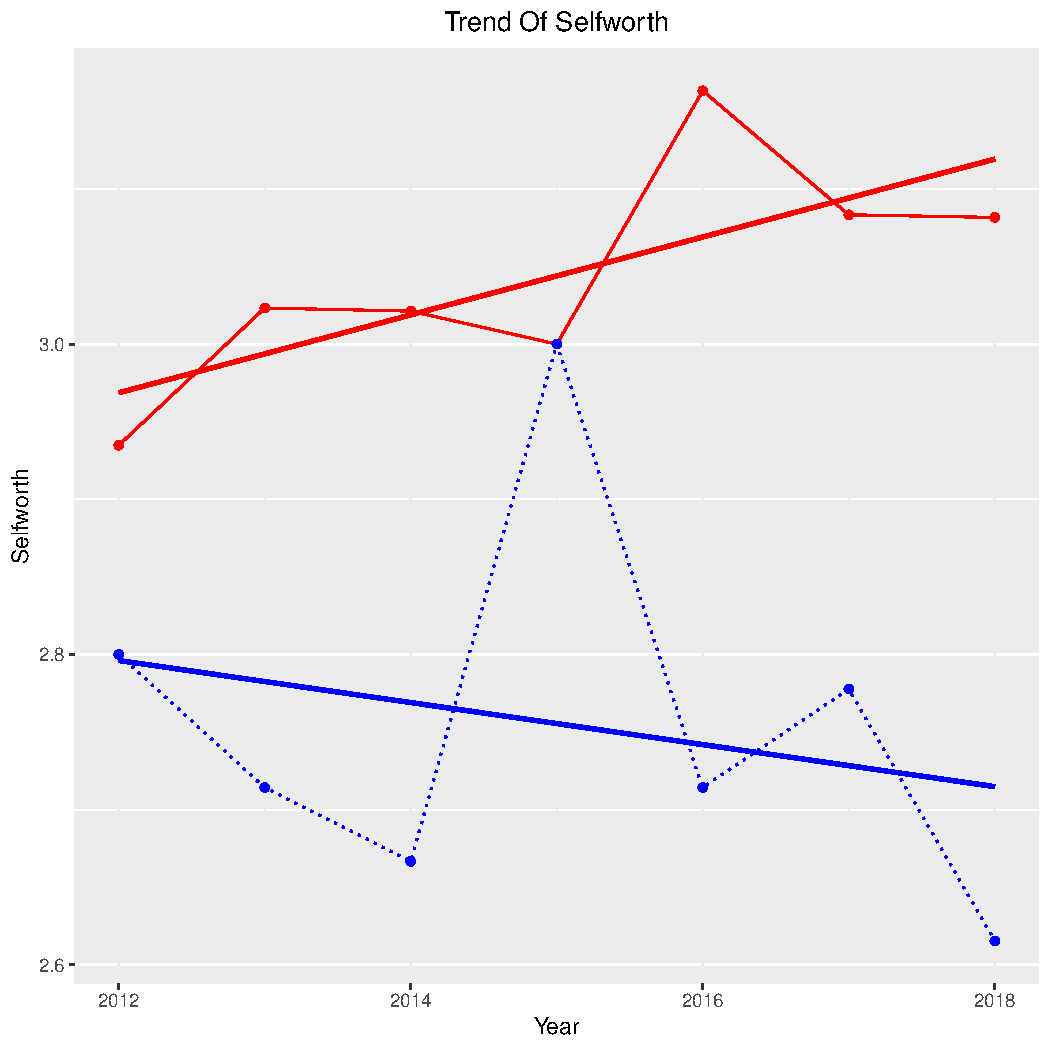
\includegraphics[width=0.8\textwidth]{figure/Selfworth-1} 

}



\end{knitrout}

\floatfoot{Note: The x-axis represents the years from 2012 to 2018, the year 2011 is left out because the trips program starts in 2012. The y-axis represents the average answers from the organizations regarding to selfworth. The time trend of the average answers of the organizations in the treatment group is characterised by the solid red line, the answers of the control group by the dotted blue line. Additionally, the linear trends of both groups are included as the straight lines.}
\end{figure}

\begin{figure}
  \caption{Trend in share of beneficiaries with broadened everyday competence}
  \label{dayToDaySkills_Trend}

\begin{knitrout}
\definecolor{shadecolor}{rgb}{0.969, 0.969, 0.969}\color{fgcolor}

{\centering 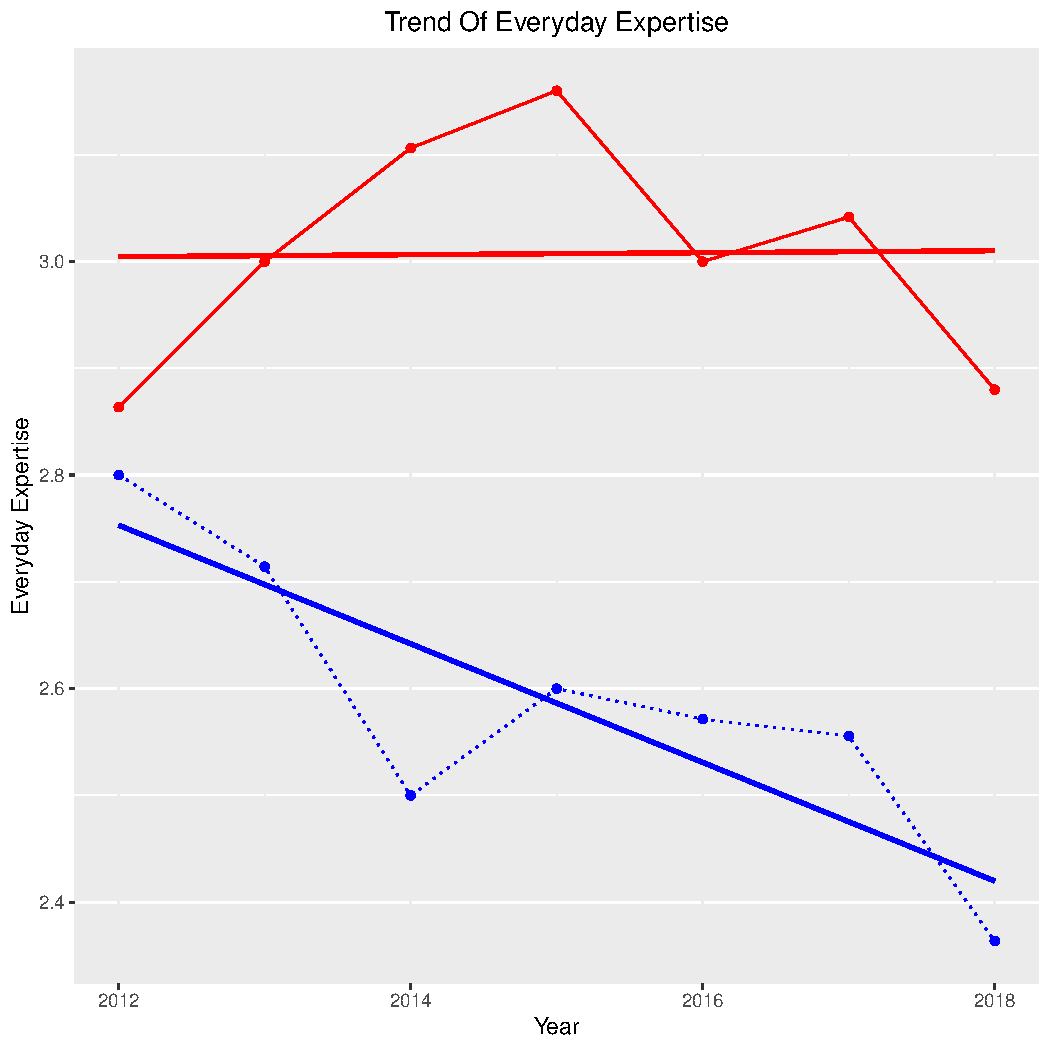
\includegraphics[width=0.8\textwidth]{figure/Daytodayskills-1} 

}



\end{knitrout}

\floatfoot{Note: The x-axis represents the years from 2012 to 2018, the year 2011 is left out because the trips program starts in 2012. The y-axis represents the average answers from the organizations regarding to everyday expertise. The time trend of the average answers of the organizations in the treatment group is characterised by the solid red line, the answers of the control group by the dotted blue line. Additionally, the linear trends of both groups are included as the straight lines.}
\end{figure}

To check for differences in treatment and control group, we created descriptive statistics regarding to the variables of interest.
Figure 5 and Figure 6 represent the development of average selfworth and average everyday expertise over time for both the treatment and control group. The two graphs illustrate a difference in levels as well as in trends between the treatment and control group in either average selfworth or average everyday expertise. In the treatment group the average selfworth increased over time  while it decreased in the control group (Figure 5). Moreover, average everyday expertise declines in the control group over time while it remains constant in the treatment group (Figure 6). The divergence shown in both graphs suggests that funding for the trips program might positively influence the selfworth and everyday expertise of participating children and adolescents. This evidence could support the hypothesis that the trips program positively influences the beneficiaries. However, this graphical analysis is only descriptive and therefore cannot be interpreted as a causal relationship.

\subsubsection{Differences-in-Differences Estimation}

For the empirical analysis, we implement a differences-in-differences (DID) strategy to test whether the trips program has a positive influence on the selfworth and everyday expertise of the supported children. The DID estimator measures the effect of participating in the trips program by comparing the changes in dependent variables over time between the treatment and control group. The key identifying assumption for the DID strategy is the common trend assumption. The assumption states that, in the absence of the trips program, both the treatment and control group would have evolved with the same trend meaning that the difference between the groups would have stayed the same. In case of a violation of the parallel trend assumption, the estimated treatment effect would be biased. As the dataset contains 2011 as the only year in the pre-period, we are not able to observe a pre-trend. Therefore, we cannot argue that the common trend assumption is fulfilled.

Using the panel structure of the dataset we implement the DID estimation with the following regression equation:
\begin{equation}
\label{didregression}
  Y_{it} = \alpha + \beta \cdot TreatEF_{it} + \gamma_{i} + \delta_{t} + \epsilon_{it}
\end{equation}

where $i$ indexes the identification number of each organization supported by CHILDREN and $t$ indexes the year of observation. The outcome variable, denoted by $Y_{it}$, is either selfworth or everyday expertise. As mentioned in the previous section, $TreatEF_{it}$ represents the treatment status of organization $i$ in year $t$. The corresponding regression coefficient $\beta$ represents the DiD estimator, which measures the average treatment effect of participating in the trips program.

The panel data set allows us to implement fixed effects. In our analysis we introduce individual fixed effects and time fixed effects. The ID fixed effects $\gamma_{i}$ control for organization specific observable and unobservable characteristics that are constant over time but differ across social institutions. For example, the state of an organization does not vary over time but might differ across supported social institutions. Additionally, the year fixed effects $\delta_{t}$ capture all variables that change across years but are the same for all organizations and within a specific year. For all following regression estimations, we use robust standard errors to take potential heteroscedasticity into account.

One concern with our empirical approach is that the allocation to treatment and control group might not be perfectly randomized because the selection into the treatment could be driven by time-variant characteristics. Therefore, we include a set of control variables to deal with potential selection bias. For this, we select variables of the available dataset that might influence both the treatment status and either of the outcome variables. Furthermore, we control for organization specific characteristics which include the subsidy received for the meals program, the corresponding total costs of providing meals and the number of days in a week on which children cook in a specific social institution.

\subsection{Results}

\subsubsection{Everyday Expertise}

The estimated coefficients of equation 4 are represented in Table \ref{table:coefficients1} with everyday expertise as the dependent variable. Columns (1)-(2) report estimates using the first definition of the treatment variable, while columns (3)-(4) apply the second treatment specification. Columns (1) and (3) only include ID fixed effects and year fixed effects without any controls. Columns (2) and (4) expand the regression equation by adding the organization specific control variables: Subsidy, total costs and the number of days in a week on which children cook in a social institution.


\begin{table}
\begin{center}
\begin{tabular}{l c c c c}
\\[-1.8ex]\hline
& \multicolumn{4}{c}{\textit{Dependent variable:}} \\
\cline{2-5}
\\[-1.8ex] & \multicolumn{4}{c}{Everyday Expertise} \\
\hline
 & (1) & (2) & (3) & (4) \\
\hline
treatEF                & $-0.010$  & $-0.166$     & $0.247$   & $0.255$      \\
                       & $(0.326)$ & $(0.405)$    & $(0.299)$ & $(0.310)$    \\
subsidy                &           & $0.019$      &           & $0.016$      \\
                       &           & $(0.014)$    &           & $(0.014)$    \\
totalCost              &           & $0.001^{**}$ &           & $0.001^{*}$  \\
                       &           & $(0.000)$    &           & $(0.000)$    \\
weeklyCooks            &           & $0.166^{**}$ &           & $0.162^{**}$ \\
                       &           & $(0.072)$    &           & $(0.073)$    \\
\hline
ID fixed effects       & $Yes$     & $Yes$        & $Yes$     & $Yes$        \\
Year fixed effects     & $Yes$     & $Yes$        & $Yes$     & $Yes$        \\
Number of observations & $428$     & $410$        & $428$     & $410$        \\
R$^2$                  & $0.475$   & $0.490$      & $0.476$   & $0.491$      \\
\hline
\multicolumn{5}{l}{\scriptsize{$^{***}p<0.01$; $^{**}p<0.05$; $^{*}p<0.1$}}
\end{tabular}
\caption{DID Estimation: Results for Everyday Expertise}
\label{table:coefficients1}
\end{center}
\end{table}



Using the first definition of the treatment variable, the average treatment effect of participating in the trips program on everyday expertise is negative, but not statistically significant. Therefore, the estimated coefficient in column (1) implies that the trips program would not have a significant effect on everyday expertise of the supported children and adolescents. However, this negative estimate could result from the fact that we consider several organizations as treated even though they did not receive funding for the trips program in a given year. As a result, the number of observation units in the control group is reduced so that the difference in size between the treatment and control group is considerably high. Therefore, this finding should not be overstated. On the other hand, using the alternative specification of the treatment indicator in column (3), the average treatment effect is positive, but remains insignificant. Thus, the sign of the estimated treatment effect changes if we use the alternative definition of the treatment variable. With the second treatment variable, the number of organizations in the control group increases, as the treatment status depends on actually receiving funding in a given year. Nevertheless, the difference in size of the treatment and control group remains relatively large. However, the estimate in Column (3) could provide evidence that the treatment effect might be positive and potentially turn significant if the sample size increases.

Adding the organization specific control variables in Column (2) and Column (4) does not influence the size of both effects and the significance substantially.

\subsubsection{Selfworth}

Using selfworth as the outcome variable, the estimates of regression equation \ref{didregression} are reported in Table \ref{table:coefficients2}, whose structure is equal to Table \ref{table:coefficients1}.

\begin{table}
\begin{center}
\begin{tabular}{l c c c c}
\\[-1.8ex]\hline
& \multicolumn{4}{c}{\textit{Dependent variable:}} \\
\cline{2-5}
\\[-1.8ex] & \multicolumn{4}{c}{Selfworth} \\
\hline
 & (1) & (2) & (3) & (4) \\
\hline
treatEF                & $-0.474$  & $-0.481$  & $-0.328$  & $-0.442^{*}$ \\
                       & $(0.309)$ & $(0.312)$ & $(0.247)$ & $(0.256)$    \\
subsidy                &           & $0.011$   &           & $0.014$      \\
                       &           & $(0.018)$ &           & $(0.017)$    \\
totalCost              &           & $0.000$   &           & $0.000$      \\
                       &           & $(0.001)$ &           & $(0.001)$    \\
weeklyCooks            &           & $0.036$   &           & $0.037$      \\
                       &           & $(0.069)$ &           & $(0.069)$    \\
\hline
ID fixed effects       & $Yes$     & $Yes$     & $Yes$     & $Yes$        \\
Year fixed effects     & $Yes$     & $Yes$     & $Yes$     & $Yes$        \\
Number of observations & $428$     & $410$     & $428$     & $410$        \\
R$^2$                  & $0.475$   & $0.484$   & $0.474$   & $0.485$      \\
\hline
\multicolumn{5}{l}{\scriptsize{$^{***}p<0.01$; $^{**}p<0.05$; $^{*}p<0.1$}}
\end{tabular}
\caption{DID Estimation: Results for Selfworth}
\label{table:coefficients2}
\end{center}
\end{table}

Strinkinlgy, all columns of Table \ref{table:coefficients2} report a negative treatment effect, regardless of the definition of the treatment variable or the inclusion of organization specific controls. In column (1)-(3), the average treatment effect is insignificant. However, the estimated effect is significant if we use the second specification of the treatment status and include controls in column (4). This indicates that participating in the trips program would negatively influence the selfworth of the children and adolescents. This surprising result contradicts our hypothesis that the participation in the trips program positively influences the selfworth of the beneficiaries. As previously mentioned, the number of observation units in both treatment and control group is relatively small. Therefore, this unexpected negative effect of the trips program on selfworth should not be overstated. Moreover, another possible explanation for the observed results could be that the survey questions are answered by employees of an organization and not by the children and adolescents themselves. It might be difficult for the respondents of the survey to assess children specific characteristics, such as selfworth. During our visit in Augsburg, the employees confirmed that it is challenging to evaluate the variables asked in the survey for all participants in the entire social institution, especially with a lot of variation in attendance. One potential solution for this problem could be to directly ask the children and adolescents. Data on the individual level might be more precise because the children could assess themselves better. When using variables on the level of beneficiaries, we might observe a positive effect of the trips program on selfworth.
As reported in the summary statistics, the outcome variable shows a low variation. This results from the fact that, most of the time, organizations give the answer “all children” and “most children” when asked about the improvement of children’s selfworth. In general, it is more unlikely to find significant effects if the variation of the dependent variable is low. Therefore, one challenge for further analysis is to ask for variables that have a potentially higher variation.

\section{Conclusion}

Until now CHILDREN only influences whether organizations are supported and how much funding they receive to provide both the trips and the meals program. However, we find a strong positive correlation between the healthiness of the meals that organizations serve and health related outcomes of children and adolescents. During our visit of an organization in Augsburg, the employees told us that both the children and adolescents appreciate the healthy food and demand even more healthier meals. This might be one possible way for CHILDREN to improve the beneficiaries’ health without the necessity of spending particularly more money. In the yearly meetings, they could point out our results and mention their appreciation of the provision of healthy food. Moreover, CHILDREN could request that the organizations fulfill the DGE criteria for the provided meals. Due to the good relationship between CHILDREN and the supported social institutions, we think that the organizations are open to implementing this proposal.

On the basis of the processed dataset, we cannot measure the causal effect of the trips program on everyday expertise and selfworth of beneficiaries. However, measuring significant effects of CHILDREN’s trips program might be possible if the data structure will be adjusted. At this point, we recommend to directly ask the beneficiaries to answer the children specific questions of the survey. During our first meeting with CHILDREN we were informed that they already have collected data from children and adolescents directly, that caused additional workload. For instance, the organizations need to obtain the permission of the parents. Nevertheless, the individual level data are perhaps more precise.

The dataset contains several helpful features that made our analysis easier. For example, CHILDREN has asked for many survey questions from the supported organizations in every year across the whole observation period. Furthermore, the dataset includes variables regarding increased selfworth and broadened everyday expertise for both programs allowing a comparison of the meals and the trips program. Hence, we recommend to continue asking the same questions in every year and selected variables for both programs. 


\printbibliography

\section{Appendix}

\subsection{A1: Expanded Health Regression}

In addition to table \ref{HealthRegressions-LessIll}, table \ref{expandLessIll} presents the results of an OLS approach with scaled outcomes as well as a WLS approach with scaled outcomes with following control variables: to which extent an organization uses regional products, since when an organization is part of the Lunch program, the real subsidy per beneficiary and the state an organization is located. In comparison to the simple linear model, there are only small changes in coefficents. 

% <<eqaulity_extra_reg, echo=FALSE, results='asis', message=FALSE, warning=FALSE>>=
% 
% lm_s = readRDS("./ANALYSIS/Tables/selfworth.lm.Rds") #weighted
% lm_d = readRDS("./ANALYSIS/Tables/dayToDaySkills.lm.Rds") #weighted
% ts = readRDS("./ANALYSIS/Tables/selfworthTrips.lm.Rds")
% td = readRDS("./ANALYSIS/Tables/dayToDaySkillsTrips.lm.Rds")
% sI = readRDS("./ANALYSIS/Tables/selfworth_IM.lm.Rds") #weighted
% dI = readRDS("./ANALYSIS/Tables/dayToDaySkills_IM.lm.Rds") #weighted
% tsI = readRDS("./ANALYSIS/Tables/selfworthTrips_IM.lm.Rds")
% tdI = readRDS("./ANALYSIS/Tables/dayToDaySkillsTrips_IM.lm.Rds")
% @


\usepackage{graphicx}

\begin{table}
\begin{center}
\scalebox{0.8}{
\begin{tabular}{l c c c c}
\hline
 & OLS & WLS & OLS Impute & WLS Impute \\
\hline
(Intercept)               & $-1.08^{***}$ & $-0.99^{**}$ & $-0.04$      & $-0.08$    \\
                          & $(0.24)$      & $(0.30)$     & $(0.18)$     & $(0.20)$   \\
DGECriteriaNoScaled       & $0.34^{***}$  & $0.36^{***}$ & $0.23^{***}$ & $0.27$     \\
                          & $(0.08)$      & $(0.06)$     & $(0.07)$     & $(0.14)$   \\
regionalProducts\_scaled  & $0.02$        & $-0.03$      & $0.11$       & $0.02$     \\
                          & $(0.08)$      & $(0.11)$     & $(0.07)$     & $(0.11)$   \\
yearsSupportSince         & $0.02$        & $-0.03$      & $0.01$       & $0.05^{*}$ \\
                          & $(0.03)$      & $(0.04)$     & $(0.02)$     & $(0.02)$   \\
realSubsidyPerBeneficiary & $-0.00$       & $0.00$       & $0.00$       & $-0.00$    \\
                          & $(0.00)$      & $(0.00)$     & $(0.00)$     & $(0.00)$   \\
stateBayern               & $0.96^{**}$   & $1.88^{***}$ &              &            \\
                          & $(0.33)$      & $(0.49)$     &              &            \\
stateBerlin               & $1.09^{**}$   & $1.34^{***}$ &              &            \\
                          & $(0.37)$      & $(0.37)$     &              &            \\
stateBrandenburg          & $2.21^{***}$  & $2.46^{***}$ &              &            \\
                          & $(0.43)$      & $(0.40)$     &              &            \\
stateBremen               & $1.00$        & $1.03$       &              &            \\
                          & $(0.58)$      & $(0.59)$     &              &            \\
stateHamburg              & $0.95$        & $1.96^{***}$ &              &            \\
                          & $(0.67)$      & $(0.40)$     &              &            \\
stateHessen               & $0.87^{***}$  & $1.16^{***}$ &              &            \\
                          & $(0.23)$      & $(0.31)$     &              &            \\
stateMV                   & $0.09$        & $0.14$       &              &            \\
                          & $(0.21)$      & $(0.26)$     &              &            \\
stateNiedersachsen        & $2.48^{***}$  & $2.30^{***}$ &              &            \\
                          & $(0.40)$      & $(0.43)$     &              &            \\
stateNRW                  & $0.68^{*}$    & $1.00^{**}$  &              &            \\
                          & $(0.27)$      & $(0.33)$     &              &            \\
stateSaarland             & $1.50^{***}$  & $1.75^{***}$ &              &            \\
                          & $(0.32)$      & $(0.25)$     &              &            \\
stateSachsen              & $1.34^{***}$  & $1.23^{***}$ &              &            \\
                          & $(0.27)$      & $(0.27)$     &              &            \\
stateSchleswig-Holstein   & $1.33^{***}$  & $1.63^{***}$ &              &            \\
                          & $(0.37)$      & $(0.42)$     &              &            \\
stateThüringen            & $0.99$        & $1.29^{*}$   &              &            \\
                          & $(0.59)$      & $(0.55)$     &              &            \\
\hline
R$^2$                     & $0.51$        & $0.73$       & $0.09$       & $0.22$     \\
Adj. R$^2$                & $0.39$        & $0.66$       & $0.07$       & $0.20$     \\
Num. obs.                 & $88$          & $88$         & $175$        & $175$      \\
RMSE                      & $0.73$        & $5.62$       & $0.94$       & $7.77$     \\
\hline
\multicolumn{5}{l}{\scriptsize{\parbox{\linewidth}
{\vspace{2pt} Dependent variable: share of beneficiaries who are less frequently ill \\ DGECriteriaNo: index of healthy diet criteria fulfilled in organization's menu \\ regionalProducts: wether the organization offers meals with local ingredients or not \\ yearsSupportSince: the number of years an organization is already part of the Meals program \\ realSubsidyPerBeneficiary: subsidy per beneficiary of Meals program in 2015 EUR \\ state: german 'Bundeland' \\ Model (1): original data set, simple linear model with controls, estimated with OLS \\ Model (2): original data set, simple linear model with controls, estimated with WLS \\ Model (3): imputed data set, simple linear model with controls, estimated with OLS \\ Model (4): imputed data set, simple linear model with controls, estimated with WLS \\ All regressions are estimated with robust standard errors $^{***}p<0.001$; $^{**}p<0.01$; $^{*}p<0.05$.}}}
\end{tabular}
}
\caption{Regression Results: Less ill expanded model}
\label{expandLessIll}
\end{center}
\end{table}


\subsection{A2: Cumulative Odds Regression} 

As an option to run a regression on the original ordinal variables, we use the proportional odds version of the cumulative logit. Equation \ref{PropoddsModel} describes the model setup: 

 
\begin{equation}
\label{PropoddsModel}
  P(Y_i \leq \ r) = \frac{exp(y_{0r} + x_i^Ty)}{1+exp(y_{0r} + x_i^Ty)}    
\end{equation}


To demonstrate the results of this method, we show in the tables \ref{lessIllOdds}, \ref{dietaryOdds}, \ref{appreciateOdds} the regressions of the health related variables on the healthy meals criterion and in the tables \ref{selfworthOdds} and \ref{dayToDayOdds} the regressions of the real meals subsidy on selfworth and everyday expertise. 

As an example of interpreting such models, we consider the model of table \ref{lessIllOdds}: An increase of the healthy meals criterion by 1 is associated with an increase in chances, that a proportion of a maximum of r beneficiaries is healthier in relation to that a proportion of more than r beneficiaries are healthier, by the factor of exp(-0.29127) = 0.75.

A summary of the remaining models:

\begin{itemize}
  \item{Dietary Knowledge: exp(-0.089) = 0.91}
  \item{Appreciate Healthy: exp(-0199) = 0.82}
  \item{Selfworth: exp(-0.00001) = 1}
  \item{Everyday Expertise: (-0.00003) = 1} 
\end{itemize}

\begin{kframe}


{\ttfamily\noindent\color{warningcolor}{\#\# Warning: namespace 'VGAM' is not available and has been replaced\\\#\# by .GlobalEnv when processing object ''}}\end{kframe}
% Table created by stargazer v.5.2.2 by Marek Hlavac, Harvard University. E-mail: hlavac at fas.harvard.edu
<<<<<<< HEAD
% Date and time: Sa, Feb 29, 2020 - 17:56:48
=======
% Date and time: Sa, Feb 29, 2020 - 17:58:55
>>>>>>> b24662a116b8b0301ff26431155b33d6392d6dc5
% Requires LaTeX packages: dcolumn 
\begin{table}[!htbp] \centering 
  \caption{Propodss Regression Results: Association of index of healthy diet criteria fulfilled in organization's menu and the share of beneficiaries who are less frequently ill} 
  \label{lessIllOdds} 
\begin{tabular}{@{\extracolsep{5pt}} D{.}{.}{-3} D{.}{.}{-3} D{.}{.}{-3} D{.}{.}{-3} D{.}{.}{-3} } 
\\[-1.8ex]\hline 
\hline \\[-1.8ex] 
\multicolumn{1}{c}{} & \multicolumn{1}{c}{Estimate} & \multicolumn{1}{c}{Std. Error} & \multicolumn{1}{c}{z value} & \multicolumn{1}{c}{Pr(\textgreater \textbar z\textbar )} \\ 
\hline \\[-1.8ex] 
\multicolumn{1}{c}{(Intercept):1} & -2.799 & 1.109 & -2.523 & 0.012 \\ 
\multicolumn{1}{c}{(Intercept):2} & 1.653 & 0.582 & 2.841 & 0.004 \\ 
\multicolumn{1}{c}{(Intercept):3} & 4.667 & 0.738 & 6.322 & 0 \\ 
\multicolumn{1}{c}{DGECriteriaNo} & -0.291 & 0.075 & -3.883 & 0.0001 \\ 
\hline \\[-1.8ex] 
\end{tabular} 
\end{table} 


\begin{kframe}


{\ttfamily\noindent\color{warningcolor}{\#\# Warning: namespace 'VGAM' is not available and has been replaced\\\#\# by .GlobalEnv when processing object ''}}\end{kframe}
% Table created by stargazer v.5.2.2 by Marek Hlavac, Harvard University. E-mail: hlavac at fas.harvard.edu
<<<<<<< HEAD
% Date and time: Sa, Feb 29, 2020 - 17:56:48
=======
% Date and time: Sa, Feb 29, 2020 - 17:58:55
>>>>>>> b24662a116b8b0301ff26431155b33d6392d6dc5
% Requires LaTeX packages: dcolumn 
\begin{table}[!htbp] \centering 
  \caption{Propodss Regression Results: Association of index of healthy diet criteria fulfilled in organization's menu and share of beneficiaries with expanded dietary knowledge} 
  \label{dietaryOdds} 
\begin{tabular}{@{\extracolsep{5pt}} D{.}{.}{-3} D{.}{.}{-3} D{.}{.}{-3} D{.}{.}{-3} D{.}{.}{-3} } 
\\[-1.8ex]\hline 
\hline \\[-1.8ex] 
\multicolumn{1}{c}{} & \multicolumn{1}{c}{Estimate} & \multicolumn{1}{c}{Std. Error} & \multicolumn{1}{c}{z value} & \multicolumn{1}{c}{Pr(\textgreater \textbar z\textbar )} \\ 
\hline \\[-1.8ex] 
\multicolumn{1}{c}{(Intercept):1} & -4.009 & 0.803 & -4.996 & 0.00000 \\ 
\multicolumn{1}{c}{(Intercept):2} & -1.047 & 0.425 & -2.465 & 0.014 \\ 
\multicolumn{1}{c}{(Intercept):3} & 1.445 & 0.430 & 3.365 & 0.001 \\ 
\multicolumn{1}{c}{DGECriteriaNo} & -0.089 & 0.052 & -1.712 & 0.087 \\ 
\hline \\[-1.8ex] 
\end{tabular} 
\end{table} 


\begin{kframe}


{\ttfamily\noindent\color{warningcolor}{\#\# Warning: namespace 'VGAM' is not available and has been replaced\\\#\# by .GlobalEnv when processing object ''}}\end{kframe}
% Table created by stargazer v.5.2.2 by Marek Hlavac, Harvard University. E-mail: hlavac at fas.harvard.edu
<<<<<<< HEAD
% Date and time: Sa, Feb 29, 2020 - 17:56:48
=======
% Date and time: Sa, Feb 29, 2020 - 17:58:55
>>>>>>> b24662a116b8b0301ff26431155b33d6392d6dc5
% Requires LaTeX packages: dcolumn 
\begin{table}[!htbp] \centering 
  \caption{Propodss Regression Results: Association of index of healthy diet criteria fulfilled in organization's menu and the share of beneficiaries with increased appreciation for a healthy diet} 
  \label{appreciateOdds} 
\begin{tabular}{@{\extracolsep{5pt}} D{.}{.}{-3} D{.}{.}{-3} D{.}{.}{-3} D{.}{.}{-3} D{.}{.}{-3} } 
\\[-1.8ex]\hline 
\hline \\[-1.8ex] 
\multicolumn{1}{c}{} & \multicolumn{1}{c}{Estimate} & \multicolumn{1}{c}{Std. Error} & \multicolumn{1}{c}{z value} & \multicolumn{1}{c}{Pr(\textgreater \textbar z\textbar )} \\ 
\hline \\[-1.8ex] 
\multicolumn{1}{c}{(Intercept):1} & -1.603 & 0.486 & -3.298 & 0.001 \\ 
\multicolumn{1}{c}{(Intercept):2} & 0.586 & 0.413 & 1.419 & 0.156 \\ 
\multicolumn{1}{c}{(Intercept):3} & 3.052 & 0.471 & 6.483 & 0 \\ 
\multicolumn{1}{c}{DGECriteriaNo} & -0.199 & 0.053 & -3.744 & 0.0002 \\ 
\hline \\[-1.8ex] 
\end{tabular} 
\end{table} 


\begin{kframe}


{\ttfamily\noindent\color{warningcolor}{\#\# Warning: namespace 'VGAM' is not available and has been replaced\\\#\# by .GlobalEnv when processing object ''}}\end{kframe}
% Table created by stargazer v.5.2.2 by Marek Hlavac, Harvard University. E-mail: hlavac at fas.harvard.edu
<<<<<<< HEAD
% Date and time: Sa, Feb 29, 2020 - 17:56:48
=======
% Date and time: Sa, Feb 29, 2020 - 17:58:55
>>>>>>> b24662a116b8b0301ff26431155b33d6392d6dc5
% Requires LaTeX packages: dcolumn 
\begin{table}[!htbp] \centering 
  \caption{Propodss Regression Results: Association of subsidy for Meals program in 2015 EUR and the share of beneficiaries with improved self-worth} 
  \label{selfworthOdds} 
\begin{tabular}{@{\extracolsep{5pt}} D{.}{.}{-3} D{.}{.}{-3} D{.}{.}{-3} D{.}{.}{-3} D{.}{.}{-3} } 
\\[-1.8ex]\hline 
\hline \\[-1.8ex] 
\multicolumn{1}{c}{} & \multicolumn{1}{c}{Estimate} & \multicolumn{1}{c}{Std. Error} & \multicolumn{1}{c}{z value} & \multicolumn{1}{c}{Pr(\textgreater \textbar z\textbar )} \\ 
\hline \\[-1.8ex] 
\multicolumn{1}{c}{(Intercept):1} & -4.855 & 0.584 & -8.315 & 0 \\ 
\multicolumn{1}{c}{(Intercept):2} & -1.268 & 0.143 & -8.893 & 0 \\ 
\multicolumn{1}{c}{(Intercept):3} & 1.514 & 0.150 & 10.109 & 0 \\ 
\multicolumn{1}{c}{realSubsidy} & -0.00001 & 0.00001 & -1.332 & 0.183 \\ 
\hline \\[-1.8ex] 
\end{tabular} 
\end{table} 


\begin{kframe}


{\ttfamily\noindent\color{warningcolor}{\#\# Warning: namespace 'VGAM' is not available and has been replaced\\\#\# by .GlobalEnv when processing object ''}}\end{kframe}
% Table created by stargazer v.5.2.2 by Marek Hlavac, Harvard University. E-mail: hlavac at fas.harvard.edu
<<<<<<< HEAD
% Date and time: Sa, Feb 29, 2020 - 17:56:48
=======
% Date and time: Sa, Feb 29, 2020 - 17:58:55
>>>>>>> b24662a116b8b0301ff26431155b33d6392d6dc5
% Requires LaTeX packages: dcolumn 
\begin{table}[!htbp] \centering 
  \caption{Propodss Regression Results: Association of subsidy for Meals program in 2015 EUR and the share of beneficiaries with broadened everyday expertise} 
  \label{dayToDayOdds} 
\begin{tabular}{@{\extracolsep{5pt}} D{.}{.}{-3} D{.}{.}{-3} D{.}{.}{-3} D{.}{.}{-3} D{.}{.}{-3} } 
\\[-1.8ex]\hline 
\hline \\[-1.8ex] 
\multicolumn{1}{c}{} & \multicolumn{1}{c}{Estimate} & \multicolumn{1}{c}{Std. Error} & \multicolumn{1}{c}{z value} & \multicolumn{1}{c}{Pr(\textgreater \textbar z\textbar )} \\ 
\hline \\[-1.8ex] 
\multicolumn{1}{c}{(Intercept):1} & -3.543 & 0.343 & -10.330 & 0 \\ 
\multicolumn{1}{c}{(Intercept):2} & -0.736 & 0.132 & -5.563 & 0.00000 \\ 
\multicolumn{1}{c}{(Intercept):3} & 1.764 & 0.157 & 11.249 & 0 \\ 
\multicolumn{1}{c}{realSubsidy} & -0.00003 & 0.00001 & -4.070 & 0.00005 \\ 
\hline \\[-1.8ex] 
\end{tabular} 
\end{table} 


\subsection{A3: Partition}

In addition to factor analysis, we have conducted another dimensionality reduction exercise called partition. This method is due to \textcite{Millstein.2020}. The authors propose it in the context of genome analysis, where high dimensionality is a perennnial statistical problem. 

Unlike exploratory factor analysis, the partition approach is deliberately designed to establish a one-to-one correspondence between the measured variables and presumed underlying variables. This means that the set of all variables is partitioned into subsets. A subset may contain only one variable. The deterministic partition algorithm is constructed in such a way as to ensure that there is a high correlation within subsets and a small correlation between. One can influence the number of subsets by manipulating a threshold limiting information loss. 

We use a threshold of 0.4, which means that the variables in each subset explain each other to at least 40 percent. It might be meaningful to decide to use only one of the featured variables in a reduced variable (or a summarizing one) for future surveys to avoid redundancy.

Table \ref{partitionmeals} shows the obtained results of the partition method for the variables of the Lunch program. It displays 10 variables which have not been reduced, and 5 reduced variables with a number of featured variables.

Table \ref{partitiontrips} does the same for the variables of the Trips program. Here, 12 variables have not been reduced, and a number of featured variables are summarized to 3 reduced variables. 

It is our impression that the partition technique results in a highly intuitive dimensionality reduction.

<<<<<<< HEAD
% latex table generated in R 3.6.2 by xtable 1.8-4 package
% Sat Feb 29 17:56:49 2020
=======
% latex table generated in R 3.5.1 by xtable 1.8-4 package
% Sat Feb 29 17:58:55 2020
>>>>>>> b24662a116b8b0301ff26431155b33d6392d6dc5
\begin{table}[ht]
\centering
\begin{tabular}{lccc}
  \hline
 & Variable, Meals & Mapping, Meals & Information, Meals \\ 
  \hline
1 & participateMore & participateMore & 1.00 \\ 
  2 & tasksLunch & tasksLunch & 1.00 \\ 
  3 & ownIdeas & ownIdeas & 1.00 \\ 
  4 & stayLonger & stayLonger & 1.00 \\ 
  5 & dietaryKnowledge & dietaryKnowledge & 1.00 \\ 
  6 & appreciateHealthy & appreciateHealthy & 1.00 \\ 
  7 & foodCulture & foodCulture & 1.00 \\ 
  8 & lessIll & lessIll & 1.00 \\ 
  9 & betterTeamwork & betterTeamwork & 1.00 \\ 
  10 & moreRegularSchoolVisits & moreRegularSchoolVisits & 1.00 \\ 
  11 & addressProblems & addressProblems & 1.00 \\ 
  12 & reduced\_var\_1 & moreConcentrated & 0.66 \\ 
  13 & reduced\_var\_1 & moreBalanced & 0.66 \\ 
  14 & reduced\_var\_2 & monthlyCooks & 0.42 \\ 
  15 & reduced\_var\_2 & weeklyCooks & 0.42 \\ 
  16 & reduced\_var\_2 & shoppers & 0.42 \\ 
  17 & reduced\_var\_2 & easyDishes & 0.42 \\ 
  18 & reduced\_var\_3 & dayToDaySkills & 0.43 \\ 
  19 & reduced\_var\_3 & moreIndependent & 0.43 \\ 
  20 & reduced\_var\_3 & selfworth & 0.43 \\ 
  21 & reduced\_var\_3 & moreOpen & 0.43 \\ 
  22 & reduced\_var\_3 & moreConfidence & 0.43 \\ 
  23 & reduced\_var\_3 & proud & 0.43 \\ 
  24 & reduced\_var\_4 & betterReading & 0.53 \\ 
  25 & reduced\_var\_4 & betterNumbers & 0.53 \\ 
  26 & reduced\_var\_4 & betterGrades & 0.53 \\ 
  27 & reduced\_var\_5 & influenceHome & 0.41 \\ 
  28 & reduced\_var\_5 & cookAtHome & 0.41 \\ 
  29 & reduced\_var\_5 & askRecipes & 0.41 \\ 
   \hline
\end{tabular}
\caption{Partition of outcomes, Meals} 
\label{partitionmeals}
\end{table}
<<<<<<< HEAD
% latex table generated in R 3.6.2 by xtable 1.8-4 package
% Sat Feb 29 17:56:49 2020
=======
% latex table generated in R 3.5.1 by xtable 1.8-4 package
% Sat Feb 29 17:58:55 2020
>>>>>>> b24662a116b8b0301ff26431155b33d6392d6dc5
\begin{table}[ht]
\centering
\begin{tabular}{lccc}
  \hline
 & Variable, Trips & Mapping, Trips & Information, Trips \\ 
  \hline
1 & tripsSuggestions & tripsSuggestions & 1.00 \\ 
  2 & tripsDecisions & tripsDecisions & 1.00 \\ 
  3 & tripsOrganization & tripsOrganization & 1.00 \\ 
  4 & tripsCostCalculation & tripsCostCalculation & 1.00 \\ 
  5 & tripsBudget & tripsBudget & 1.00 \\ 
  6 & tripsMoney & tripsMoney & 1.00 \\ 
  7 & tripsReview & tripsReview & 1.00 \\ 
  8 & tripsPublicTransport & tripsPublicTransport & 1.00 \\ 
  9 & tripsMobility & tripsMobility & 1.00 \\ 
  10 & tripsAdditionalActivities & tripsAdditionalActivities & 1.00 \\ 
  11 & tripsSelfworth & tripsSelfworth & 1.00 \\ 
  12 & tripsFrustrationTolerance & tripsFrustrationTolerance & 1.00 \\ 
  13 & reduced\_var\_1 & tripsSuccess & 0.68 \\ 
  14 & reduced\_var\_1 & tripsSelfEfficacy & 0.68 \\ 
  15 & reduced\_var\_2 & tripsNewPlaces & 0.60 \\ 
  16 & reduced\_var\_2 & tripsNewCommunities & 0.60 \\ 
  17 & reduced\_var\_2 & tripsNewIdeas & 0.60 \\ 
  18 & reduced\_var\_2 & tripsSocialSkills & 0.60 \\ 
  19 & reduced\_var\_3 & tripsSpecificSkills & 0.46 \\ 
  20 & reduced\_var\_3 & tripsDayToDaySkills & 0.46 \\ 
   \hline
\end{tabular}
\caption{Partition of outcomes, Trips} 
\label{partitiontrips}
\end{table}




\subsection{A4: DID Regression Results}

The estimated coefficients of equation \ref{didregression} are represented in Table \ref{table:coefficients3} with everyday expertise as the dependent variable and in Table \ref{table:coefficients4} with selfworth as the dependent variable. P-values are in parentheses. We observe decreasing p-values when using the second definition of the treatment variable.

\begin{table}
\begin{center}
\begin{tabular}{l c c c c}
& \multicolumn{4}{c}{\textit{Dependent variable:}} \\
\cline{2-5}
\\[-1.8ex] & \multicolumn{4}{c}{Everyday Expertise} \\
\hline
 & (1) & (2) & (3) & (4) \\
\hline
treatEF                & $-0.010$  & $-0.166$     & $0.247$   & $0.255$      \\
                       & $(0.975)$ & $(0.681)$    & $(0.409)$ & $(0.410)$    \\
subsidy                &           & $0.019$      &           & $0.016$      \\
                       &           & $(0.181)$    &           & $(0.258)$    \\
totalCost              &           & $0.001^{**}$ &           & $0.001^{*}$  \\
                       &           & $(0.048)$    &           & $(0.060)$    \\
weeklyCooks            &           & $0.166^{**}$ &           & $0.162^{**}$ \\
                       &           & $(0.022)$    &           & $(0.027)$    \\
\hline
ID fixed effects       & $YES$     & $YES$        & $YES$     & $YES$        \\
Year fixed effects     & $YES$     & $YES$        & $YES$     & $YES$        \\
Number of observations & $428$     & $410$        & $428$     & $410$        \\
R$^2$                  & $0.475$   & $0.490$      & $0.476$   & $0.491$      \\
\hline
\multicolumn{5}{l}{\scriptsize{$^{***}p<0.01$; $^{**}p<0.05$; $^{*}p<0.1$}}
\end{tabular}
\caption{DID Estimation 1}
\label{table:coefficients3}
\end{center}
\end{table}

\begin{table}
\begin{center}
\begin{tabular}{l c c c c}
& \multicolumn{4}{c}{\textit{Dependent variable:}} \\
\cline{2-5}
\\[-1.8ex] & \multicolumn{4}{c}{Selfworth} \\
\hline
 & (1) & (2) & (3) & (4) \\
\hline
treatEF                & $-0.474$  & $-0.481$  & $-0.328$  & $-0.442^{*}$ \\
                       & $(0.126)$ & $(0.125)$ & $(0.185)$ & $(0.085)$    \\
subsidy                &           & $0.011$   &           & $0.014$      \\
                       &           & $(0.540)$ &           & $(0.422)$    \\
totalCost              &           & $0.000$   &           & $0.000$      \\
                       &           & $(0.575)$ &           & $(0.446)$    \\
weeklyCooks            &           & $0.036$   &           & $0.037$      \\
                       &           & $(0.609)$ &           & $(0.591)$    \\
\hline
ID fixed effects       & $YES$     & $YES$     & $YES$     & $YES$        \\
Year fixed effects     & $YES$     & $YES$     & $YES$     & $YES$        \\
Number of observations & $428$     & $410$     & $428$     & $410$        \\
R$^2$                  & $0.475$   & $0.484$   & $0.474$   & $0.485$      \\
\hline
\multicolumn{5}{l}{\scriptsize{$^{***}p<0.01$; $^{**}p<0.05$; $^{*}p<0.1$}}
\end{tabular}
\caption{DID Estimation 2}
\label{table:coefficients4}
\end{center}
\end{table}


\section{Division of tasks}

Data preparation, fundamental dynamics: everybody\\
Factor analysis, general regresions, partition, cumulative odds model: Laura Jepsen and Rafael Schütz\\
DiD estimations and time series: Laura Huber, Jonathan Kirschner, and Yannick Zurl
\section{Ehrenwörtliche Erklärung aller Teilnehmer}


\end{document}
